%----------------------------------------------------------------
%
%  File    :  thesis.tex
%
%----------------------------------------------------------------

% --- Setup for the document ------------------------------------

%Class for a book like style:
\documentclass[11pt,a4paper,oneside]{scrbook}
%For a more paper like style use this class instead:
%\documentclass[11pt,a4paper,oneside]{thesis}

%input encoding for windows in utf-8 needed for Ä,Ö,Ü etc..:
\usepackage[utf8]{inputenc}
%input encoding for linux:
%\usepackage[latin1]{inputenc}
%input encoding for mac:
%\usepackage[applemac]{inputenc}

\usepackage[english]{babel}
% for german use this line instead:
%\usepackage[ngerman]{babel}

%needed for font encoding
\usepackage[T1]{fontenc}

% want Arial? uncomment next two lines...
%\usepackage{uarial}
%\renewcommand{\familydefault}{\sfdefault}

%some formatting packages
\usepackage[bf,sf]{subfigure}
\renewcommand{\subfigtopskip}{0mm}
\renewcommand{\subfigcapmargin}{0mm}

%For better font resolution in pdf files
\usepackage{lmodern}

\usepackage{url}

\usepackage{glossaries}
\newglossaryentry{facade}
{
    name=facade,
    description={The Facade pattern is a software design pattern that provides a simplified interface to a larger body of code, making it easier to use and understand. It is a structural pattern that involves creating a single class, known as the facade, which acts as a front-facing interface for a complex system of classes and components.}
}
\newglossaryentry{FaaS}
{
    name=FaaS,
    description={FaaS stands for Function-as-a-Service, which is a cloud computing model where developers can create and deploy small, single-purpose functions that are executed on demand, in response to events or triggers.}
}
\newglossaryentry{serverless}
{
    name=serverless,
    description={Serverless computing is a cloud computing model in which the cloud provider manages the infrastructure and automatically allocates computing resources as needed to execute and scale applications. In a serverless architecture, developers write and deploy code as small, independent functions that are triggered by specific events or requests, such as an HTTP request. The cloud provider then executes these functions on its own infrastructure, dynamically allocating computing resources and scaling automatically to meet demand. Because the cloud provider manages the infrastructure and abstracts away the underlying hardware and software, developers do not have to worry about managing servers, scaling infrastructure, or paying for idle resources, which can lead to reduced operational costs and increased agility.}
}
\newglossaryentry{WebAssembly}
{
    name=Wasm,
    description={WebAssembly (abbreviated Wasm) is a safe, portable, low-level code format designed for efficient execution and compact representation. Its main goal is to enable high performance applications on the Web, but it does not make any Web-specific assumptions or provide Web-specific features, so it can be employed in other environments as well.}
}
\newglossaryentry{V8}
{
    name=V8,
    description={V8 is a high-performance JavaScript engine developed by Google for use in their Chrome web browser and other applications. It is also used by Node.js to execute JavaScript code outside of a web browser. V8 is written in C++ and compiles JavaScript code to native machine code, providing significant performance benefits over interpreted JavaScript engines.}
}
\newglossaryentry{isolate}
{
    name=isolate,
    description={The isolates runtime runs on the V8 engine, which is the same engine that powers Chromium and Node.js. The Workers runtime also supports many of the standard APIs that most modern browsers have.}
}
\newglossaryentry{LXC-Container}
{
    name=LXC-Container,
    description={LXC (Linux Containers) is a lightweight virtualization technology that allows multiple isolated Linux systems, known as containers, to run on a single Linux host. LXC-Containers provide a way to run applications in an isolated environment with their own file system, network interface, and resource allocation. Each LXC-Container shares the host operating system kernel but runs its own isolated user space.}
}
\newglossaryentry{edge computing}
{
    name=edge computing,
    description={Edge computing is the concept of bringing computation power closer to the end consumer. Due to the lower proximity between the server and the end device, this solution reduces network latency. Typical use cases are in the Internet of Things, mobile or gaming sectors where latency plays a huge role.}
}
\newglossaryentry{cloud computing}
{
    name=cloud computing,
    description={According to the National Institute of Standards and Technology (NIST) definition of cloud computing is a model for enabling ubiquitous, convenient, on-demand network access to a shared pool of configurable computing resources (e.g., networks, servers, storage, applications, and services) that can be rapidly provisioned and released with minimal management effort or service provider interaction. This cloud model is composed of five essential characteristics, three service models, and four deployment models \cite{mell_2011_the}.}
}
\newglossaryentry{wasi}
{
    name=WASI,
    description={The WebAssembly System Interface is not a monolithic standard system interface, but is instead a modular collection of standardized APIs. None of the APIs are required to be implemented to have a compliant runtime. Instead, host environments can choose which APIs make sense for their use cases \cite{webassembly_2023_webassemblywasi}.}
}
\newglossaryentry{LLVM}
{
    name=LLVM,
    description={A toolkit used to build and optimize compilers. The LLVM Project consists of a set of modular and reusable compiler and toolchain technologies, which form a collection that can be utilized across various compilers and toolchains.}
}
\newglossaryentry{POSIX}
{
    name=POSIX,
    description={Portable Operating System Interface is a set of standards defined by the IEEE for maintaining compatibility between operating systems.}
}
\newglossaryentry{libc}
{
    name=libc,
    description={Short for C Standard Library, it is a library of standard functions that are a part of the C programming language, which define the functions used for file operations, input and output operations, string manipulation, and memory allocation etc.}
}
\newglossaryentry{JS glue code}
{
    name=JS glue code,
    description={It is the JavaScript code that bridges the gap between the compiled WebAssembly module and the browser. It is responsible for interfacing with the browser's JavaScript engine, allowing communication between the WebAssembly module and the web application.}
}

\makenoidxglossaries
%\makeglossaries

%\usepackage{latexsym}

\usepackage{geometry} % define pagesize in more detail

% --- Settings for header and footer ---------------------------------
\usepackage{scrlayer-scrpage}
\clearpairofpagestyles
%\clearscrheadfoot
\pagestyle{scrheadings}
\automark{chapter}

%Left header shows chapter and chapter name, will not display on first chapter page use \ihead*{\leftmark} to show on every page
\ihead{\leftmark} 	
%\ohead*{\rightmark}	%optional right header
\ifoot*{Sasan Jaghori}		%left footer shows student name
\ofoot*{\thepage}		%right footer shows pagination
%---------------------------------------------------------------------

\usepackage{colortbl} % define colored backgrounds for tables
\usepackage{xcolor}
\usepackage{courier} %for listings
\usepackage{listings} % nicer code formatting
\usepackage{textcomp} % for upquote

%
% ECMAScript 2015 (ES6) definition by Gary Hammock
% Reference: https://github.com/ghammock/LaTeX_Listings_JavaScript_ES6

\lstdefinelanguage[ECMAScript2015]{JavaScript}[]{JavaScript}{
  morekeywords=[1]{await, async, case, catch, class, const, default, do,
    enum, export, extends, finally, from, implements, import, instanceof,
    let, static, super, switch, throw, try},
  morestring=[b]` % Interpolation strings.
}

%
% JavaScript version 1.1 by Gary Hammock
%
% Reference:
%   B. Eich and C. Rand Mckinney, "JavaScript Language Specification
%     (Preliminary Draft)", JavaScript 1.1.  1996-11-18.  [Online]
%     http://hepunx.rl.ac.uk/~adye/jsspec11/titlepg2.htm
%

\lstdefinelanguage{JavaScript}{
  morekeywords=[1]{break, continue, delete, else, for, function, if, in,
    new, return, this, typeof, var, void, while, with},
  % Literals, primitive types, and reference types.
  morekeywords=[2]{false, null, true, boolean, number, undefined,
    Array, Boolean, Date, Math, Number, String, Object},
  % Built-ins.
  morekeywords=[3]{eval, parseInt, parseFloat, escape, unescape},
  sensitive,
  morecomment=[s]{/*}{*/},
  morecomment=[l]//,
  morecomment=[s]{/**}{*/}, % JavaDoc style comments
  morestring=[b]',
  morestring=[b]"
}[keywords, comments, strings]


\lstalias[]{ES6}[ECMAScript2015]{JavaScript}

% Requires package: color.
\definecolor{mediumgray}{rgb}{0.3, 0.4, 0.4}
\definecolor{mediumblue}{rgb}{0.0, 0.0, 0.8}
\definecolor{forestgreen}{rgb}{0.13, 0.55, 0.13}
\definecolor{darkviolet}{rgb}{0.58, 0.0, 0.83}
\definecolor{royalblue}{rgb}{0.25, 0.41, 0.88}
\definecolor{crimson}{rgb}{0.86, 0.8, 0.24}

\lstdefinestyle{JSES6Base}{
  backgroundcolor=\color{white},
  basicstyle=\ttfamily,
  breakatwhitespace=false,
  breaklines=false,
  captionpos=b,
  columns=fullflexible,
  commentstyle=\color{mediumgray}\upshape,
  emph={},
  emphstyle=\color{crimson},
  extendedchars=true,  % requires inputenc
  fontadjust=true,
  identifierstyle=\color{black},
  keepspaces=true,
  keywordstyle=\color{mediumblue},
  keywordstyle={[2]\color{darkviolet}},
  keywordstyle={[3]\color{royalblue}},
  numbers=left,
  numbersep=5pt,
  numberstyle=\tiny\color{black},
  rulecolor=\color{black},
  showlines=true,
  showspaces=false,
  showstringspaces=false,
  showtabs=false,
  stringstyle=\color{forestgreen},
  tabsize=2,
  title=\lstname,
  upquote=true  % requires textcomp
}

\lstdefinestyle{JavaScript}{
  language=JavaScript,
  style=JSES6Base,
  basicstyle=\ttfamily,
  breaklines=true
}
\lstdefinestyle{ES6}{
  language=ES6,
  style=JSES6Base,
  numbers=left,
  basicstyle=\ttfamily,
  breaklines=true
}

% Rust language

\lstdefinelanguage{Rust}{
  morekeywords=[1]{fn, break, continue, else, for, if, in, loop, match, return,
    while},
  % Literals, primitive types, and reference types.
  morekeywords=[2]{false, true, bool, char, i8, i16, i32, i64, isize, u8, u16,
    u32, u64, usize, f32, f64, str, String, Option, Some, None, Result, Ok,
    Err},
  % Built-ins.
  morekeywords=[3]{assert!, assert_eq!, assert_ne!, cfg!, column!, compile_error!,
    concat!, concat_idents!, debug_assert!, debug_assert_eq!, debug_assert_ne!,
    env!, eprint!, eprintln!, file!, format!, format_args!, include!, include_bytes!,
    include_str!, line!, module_path!, option_env!, panic!, print!, println!,
    select!, stringify!, thread_local!, try!, unimplemented!, unreachable!, vec!,
    write!, writeln!, macro_rules!, assert, assert_eq, assert_ne, cfg, column,
    compile_error, concat, concat_idents, debug_assert, debug_assert_eq,
    debug_assert_ne, env, eprint, eprintln, file, format, format_args, include,
    include_bytes, include_str, line, module_path, option_env, panic, print,
    println, select, stringify, thread_local, try, unimplemented, unreachable, vec,
    write, writeln},
  morecomment=[s]{/*}{*/},
  morecomment=[l]//,
  morecomment=[s]{/**}{*/}, % JavaDoc style comments
  morestring=[b]',
  morestring=[b]"
}[keywords, comments, strings]

\lstdefinestyle{Rusty}{
  backgroundcolor=\color{white},
  basicstyle=\ttfamily,
  breakatwhitespace=false,
  breaklines=false,
  captionpos=b,
  columns=fullflexible,
  commentstyle=\color{mediumgray}\upshape,
  emph={},
  emphstyle=\color{crimson},
  extendedchars=true,  % requires inputenc
  fontadjust=true,
  identifierstyle=\color{black},
  keepspaces=true,
  keywordstyle=\color{mediumblue},
  keywordstyle={[2]\color{darkviolet}},
  keywordstyle={[3]\color{royalblue}},
  numbers=left,
  numbersep=5pt,
  numberstyle=\tiny\color{black},
  rulecolor=\color{black},
  showlines=true,
  showspaces=false,
  showstringspaces=false,
  showtabs=false,
  stringstyle=\color{forestgreen},
  tabsize=2,
  title=\lstname,
  upquote=true  % requires textcomp
}

\lstdefinestyle{Rust}{
  language=Rust,
  style=Rusty,
  basicstyle=\ttfamily,
  breaklines=true
}

% Wasm language reference: https://github.com/frederikspang/webassembly-lstlisting/blob/master/wasm-listing.tex

\lstdefinelanguage{WebAssembly}{
  sensitive,
  otherkeywords={},
  morekeywords=[1]{i32,f32,i64,f64,anyfunc},
  keywordstyle={[1]\color{darkviolet}},
  morekeywords=[2]{0},
  keywordstyle={[2]\color{mediumblue}},
  morekeywords=[3]{add,const}
  keywordstyle={[3]\color{bluemunsell}},
  morekeywords=[4]{},
  keywordstyle={[4]\color{candypink}},
  morekeywords=[5]{module, func, param, result, global, get_global, mut, set_global, export, import, memory, data, get_local, set_local, elem, table, call,call_indirect, type, block, loop, br, br_if, br_table, return, if, then, else, end, drop, select, nop, unreachable, current_memory, grow_memory, i32.load, i32.store, i32.const, i32.add, i32.sub, i32.mul, i32.div_s, i32.div_u, i32.rem_s, i32.rem_u, i32.and, i32.or, i32.xor, i32.shl, i32.shr_s, i32.shr_u, i32.rotl, i32.rotr, i32.eq, i32.ne, i32.lt_s, i32.lt_u, i32.le_s, i32.le_u, i32.gt_s, i32.gt_u, i32.ge_s, i32.ge_u, i32.clz, i32.ctz, i32.popcnt, i32.eqz, i64.load, i64.store, i64.const, i64.add, i64.sub, i64.mul, i64.div_s, i64.div_u, i64.rem_s, i64.rem_u, i64.and, i64.or, i64.xor, i64.shl, i64.shr_s, i64.shr_u, i64.rotl, i64.rotr, i64.eq, i64.ne, i64.lt_s, i64.lt_u, i64.le_s, i64.le_u, i64.gt_s, i64.gt_u, i64.ge_s, i64.ge_u, i64.clz, i64.ctz, i64.popcnt, i64.eqz, f32.load, f32.store, f32.const, f32.add, f32.sub, f32.mul, f32.div, f32.min, f32.max, f32.copysign, f32.abs, f32.neg, f32.ceil, f32.floor, f32.trunc, f32.nearest, f32.sqrt, f32.eq, f32.ne, f32.lt, f32.le, f32.gt, f32.ge, f64.load, f64.store, f64.const, f64.add, f64.sub, f64.mul, f64.div, f64.min, f64.max, f64.copysign, f64.abs, f64.neg, f64.ceil, f64.floor, f64.trunc},
  keywordstyle={[5]\color{royalblue}},
  morekeywords=[6]{=,;},
  keywordstyle={[6]\color{forestgreen}},
  morekeywords=[7]{(,),[,],.},
  keywordstyle={[7]\color{black}},
  numberstyle=\tiny\color{black},
  rulecolor=\color{black},
  stringstyle=\color{forestgreen},
  morecomment=[s]{(;}{;)},
  morecomment=**[l][\itshape\color{mediumgray}]{;;},
}

\lstdefinestyle{Wasm}{
  language=WebAssembly,
  style=Rusty,
  basicstyle=\ttfamily,
  breaklines=true
}
 % import code listing settings

\usepackage{graphicx}
  \pdfcompresslevel=9
  \pdfpageheight=297mm
  \pdfpagewidth=210mm
  \usepackage[         % hyperref should be last package loaded
    pdftex, 		   % needed for pdf compiling, DO NOT compile with LaTeX
    bookmarks,
    bookmarksnumbered,
    linktocpage,
    pagebackref,
    pdfview={Fit},
    pdfstartview={Fit},
    pdfpagemode=UseOutlines,                 % open bookmarks in Acrobat
  ]{hyperref}
\DeclareGraphicsExtensions{.pdf,.jpg,.png}
\usepackage{bookmark}



\usepackage[title]{appendix}

%paper format
\geometry{a4paper,left=30mm,right=25mm, top=30mm, bottom=30mm}

\setlength{\parskip}{3pt plus 1pt minus 0pt}       % vert. space before a paragraph

\setcounter{tocdepth}{1}        % lowest section level entered in ToC
\setcounter{secnumdepth}{2}     % lowest section level still numbered

%package to force the position of the figures
\usepackage{float}

%Start of your document beginning with title page
\begin{document}
\frontmatter

% --- Main Title Page ------------------------------------------------
\begin{titlepage}
\begin{picture}(50,50)
\put(-70,40){\hbox{
\includegraphics{images/logo.png}}}
\end{picture}

\vspace*{-5.8cm}

\begin{center}

\vspace{6.2cm}

\hspace*{-1.0cm} {\LARGE \textbf{Efficient Serverless Computing with WebAssembly\\}}
\vspace{0.2cm}
%\hspace*{-1.0cm} Subtitle\\

\vspace{2.0cm}

\hspace*{-1.0cm} { \textbf{Master Thesis\\}}

\vspace{0.65cm}

\hspace*{-1.0cm} Submitted in partial fulfillment of the requirements for the degree of \\

\vspace{0.65cm}

\hspace*{-1.0cm} \textbf{Master of Science in Engineering\\}

\vspace{0.65cm}

\hspace*{-1.0cm} to the University of Applied Sciences FH Campus Wien \\
\vspace{0.2cm}
\hspace*{-1.0cm} Master Degree Program: Software Design and Engineering \\

\vspace{1.6cm}

\hspace*{-1.0cm} \textbf{Author:} \\
\vspace{0.2cm}
\hspace*{-1.0cm} Sasan Jaghori, B.Sc \\

\vspace{0.7cm}

\hspace*{-1.0cm} \textbf{Student identification number:}\\
\vspace{0.2cm}
\hspace*{-1.0cm} 2110838018 \\

\vspace{0.7cm}

\hspace*{-1.0cm} \textbf{Supervisor:} \\
\vspace{0.2cm}
\hspace*{-1.0cm} Dipl.-Ing. Georg Mansky-Kummert \\

\vspace{0.7cm}

% Reviewer if needed:
%\hspace*{-1.0cm} \textbf{Reviewer: (optional)} \\
%\vspace{0.2cm}
%\hspace*{-1.0cm} Title first name surname \\


\vspace{1.0cm}

\hspace*{-1.0cm} \textbf{Date:} \\
\vspace{0.2cm}
\hspace*{-1.0cm} 31.05.2023 \\

\end{center}
\end{titlepage}

\newpage

\setcounter{page}{1}

\vspace*{16cm}

% --- Declaration of authorship ----------------------------------------------------
\hspace*{-0.7cm} \underline{Declaration of authorship:}\\\\
I declare that this Master Thesis has been written by myself. I have not used any other than the listed sources, nor have I received any unauthorized help.\\\\
I hereby certify that I have not submitted this Master Thesis in any form (to a reviewer for assessment) either in Austria or abroad.\\\\
Furthermore, I assure that the (printed and electronic) copies I have submitted are identical.
\\\\\\
Date: \hspace{6cm} Signature:\\

% --- English Abstract ----------------------------------------------------
\cleardoublepage
\chapter*{Abstract}
In recent years, serverless computing has emerged as a popular paradigm for building scalable and cost-efficient cloud applications. However, this paradigm was not sufficient for latency-critical applications in the IoT, mobile, or gaming segments due to cold-start latencies. An edge computing paradigm has emerged to address this issue, which places cloud provider servers closer to customers to improve latency. However, using existing virtualization techniques, the problem of cold starts remains a challenge in edge computing. Furthermore, limited CPU power and memory resources in the host environment can further increase latencies, making it difficult to achieve the desired performance for latency-critical applications. 

Because of these challenges, there is a need for an execution environment that doesn't have cold start latencies and is as secure as traditional containerization technologies and micro virtual machines such as Firecracker used by serverless cloud providers. One promising technology is WebAssembly. Initially designed as a common compilation target in the browser, it has shown that the same technology can be used in the server environment as well. It is lightweight, language-agnostic, cross-platform, secure, and fast.

The aim of this thesis is to assess whether the usage of WebAssembly technology will satisfy the challenging requirements of the edge computing paradigm, allowing us to build applications that depend on fast response times. For this, we evaluate the performance of WebAssembly engines and consider various factors that affect performance and usability, among other things. 

We use both microbenchmarks and macrobenchmarks to evaluate the performance of \hbox{WebAssembly} runtimes and existing serverless offerings. Through microbenchmarks, we find that the instantiation time is about 40 microseconds compared to alternatives such as Firecracker's microVM, which takes about 125 milliseconds. The results demonstrate that using WebAssembly in the serverless environment represents significant progress towards enabling a wide range of latency-critical applications.


% --- German Abstract ----------------------------------------------------

\cleardoublepage
\chapter*{Kurzfassung}
In den letzten Jahren hat sich das serverlose Computing zu einem beliebten Paradigma für die Erstellung skalierbarer und kosteneffizienter Cloud-Anwendungen entwickelt. Dieses Paradigma war jedoch für latenzkritische Anwendungen im IoT-, Mobil- oder Spielesegment aufgrund von Kaltstartlatenzzeiten nicht ausreichend. Zur Lösung dieses Problems hat sich ein Edge-Computing-Paradigma herausgebildet, bei dem die Server der Cloud-Anbieter näher am Kunden platziert werden, um die Latenzzeit zu verbessern. Bei der Verwendung bestehender Virtualisierungstechniken bleibt das Problem der Kaltstarts jedoch eine Herausforderung beim Edge Computing. Darüber hinaus können begrenzte CPU-Leistung und Speicherressourcen in der Host-Umgebung die Latenzzeiten weiter erhöhen, was es schwierig macht, die gewünschte Leistung für latenzkritische Anwendungen zu erreichen. 

Aufgrund dieser Herausforderungen besteht ein Bedarf an einer Ausführungsumgebung, die keine Kaltstartlatenzen aufweist und ebenso sicher ist wie herkömmliche Containerisierungstechnologien und "microVMs" wie Firecracker, die von serverlosen Cloud-Anbietern verwendet werden. Eine vielversprechende Technologie ist WebAssembly. Ursprünglich als gemeinsames Kompilierungsziel im Browser entwickelt, hat sie gezeigt, dass dieselbe Technologie auch in der Serverumgebung eingesetzt werden kann. Sie ist leichtgewichtig, sprachunabhängig, plattformübergreifend, sicher und schnell.

In dieser Arbeit soll untersucht werden, ob die Verwendung der WebAssembly-Technologie den anspruchsvollen Anforderungen des Edge-Computing-Paradigmas gerecht wird und es uns ermöglicht, Anwendungen zu entwickeln, die auf schnelle Antwortzeiten angewiesen sind. Zu diesem Zweck bewerten wir die Leistung von WebAssembly-Engines und berücksichtigen verschiedene Faktoren, die unter anderem die Leistung und die Benutzerfreundlichkeit beeinflussen. 

Wir verwenden sowohl Mikrobenchmarks als auch Makrobenchmarks, um die Leistung von \hbox{WebAssembly}-Laufzeiten und bestehenden serverlosen Angeboten zu bewerten. Durch Mikrobenchmarks finden wir heraus, dass die Instanziierungszeit etwa 40 Mikrosekunden beträgt, verglichen mit Alternativen wie Firecrackers microVM, die etwa 125 Millisekunden benötigt. Die Ergebnisse zeigen, dass die Verwendung von WebAssembly in der Serverless-Umgebung einen bedeutenden Fortschritt bei der Ermöglichung eines breiten Spektrums an latenzkritischen Anwendungen darstellt.


% --- Abbrevations ----------------------------------------------------
\newpage\noindent
\chapter*{List of Abbreviations}
\vspace{0.65cm}

\begin{table*}[htbp]
		\begin{tabular}{ll}
			AOT & Ahead-of-time compilation \\
			DOM & Document Object Model \\
   			JIT & Just-in-time compilation \\
			LLVM & Low Level Virtual Machine \\
			POSIX & Portable Operating System Interface \\
			SIMD & Single Instruction Multiple Data \\
   			VM & Virtual Machine \\
			WASM & WebAssembly \\
			WASI & WebAssembly System Interface \\
			WAT  &  WebAssembly Text Format \\
			WIT  &  WebAssembly Interface Type \\  
		\end{tabular}
\end{table*}

% --- Key terms ----------------------------------------------------
\newpage
\chapter*{Key Terms}
\vspace{0.65cm}

\begin{itemize}
	\setlength{\itemsep}{0pt}
	\item[] WASM
	\item[] WebAssembly
	\item[] Serverless
	\item[] Edge Computing
	\item[] Cloud Computing
	\item[] AWS Lambda
 	\item[] FaaS
 	\item[] Web Engineering
\end{itemize}

% --- Table of contents autogenerated ------------------------------------
\newpage
\tableofcontents

% --- Begin of Thesis ----------------------------------------------------
\mainmatter
\chapter{Introduction}
\label{chap:intro}

In recent years, \gls{serverless} computing has emerged as a popular paradigm for building scalable and cost-efficient cloud applications. \Gls{serverless} platforms allow developers to focus on writing code without worrying about server management or infrastructure scaling, while users only pay for the computing time.

While \gls{serverless} computing is an effective model for managing unpredictable and bursty
workloads, it has limitations in supporting latency-critical applications in the IoT, mobile or gaming segments due to cold-start latencies of several hundred milliseconds or more \cite{gackstatter_2022_pushing}. 

An \gls{edge computing} paradigm has emerged to address this issue, which places cloud providers closer to customers to improve latency. However, the issue of cold starts remains a challenge in edge computing. Furthermore, limited CPU power and memory resources in the host environment can further increase latencies, making achieving the desired performance for latency-critical applications difficult.

The underlying issue can be referred to the current runtime environments for \gls{serverless} functions, which primarily rely on \Gls{LXC-Container} technologies like Docker or microVMs like Firecracker. To address these challenges, a more innovative approach would be to execute users' code efficiently and minimize cold start impacts, for instance by replacing heavier containers with lighter alternatives that maintain the advantages of container isolation.

The same requirements for isolation, fast execution and security apply to WebAssembly as well. WebAssembly (\Gls{WebAssembly}) has gained traction as a portable binary format that is executed in an isolated sandbox environment. Wasm is a compilation target, originally designed for browser applications to run e.g. C++ compiled code at near-native speed. This makes WebAssembly the perfect candidate for server-side code execution especially for serverless computing where startup times play a huge role. However, while Wasm was developed with browser execution in mind, standardized system APIs are needed to enable its use on the server side in order to access basic system resources like standard output or file input. Bytecode Alliance is working on the WebAssembly standard and a system interface standard called WASI \cite{webassembly_2023_webassemblywasi}.

\begin{figure}[H]
	\centering
		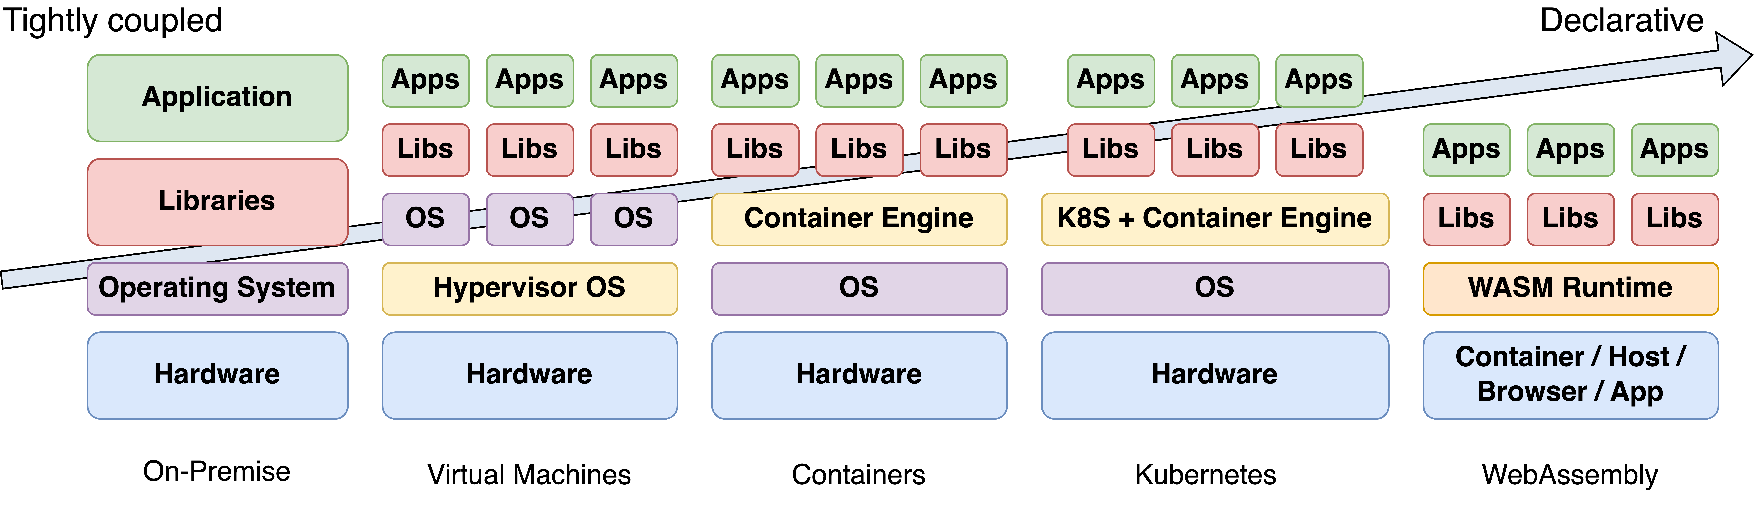
\includegraphics[width=\textwidth,height=\textheight,keepaspectratio]{images/introduction/Cloud_Transformation.pdf}
	\caption{Evolution of computation from on-premise to Wasm based on \cite{randall_2021_wasmcloud}}
	\label{fig:cloud-transformation}
\end{figure}

The figure \ref{fig:cloud-transformation} below depicts the evolution of \gls{cloud computing} from on premise model to the described WebAssembly serverless model.

Another promising browser technology is the usage of \gls{V8} \glspl{isolate}. According to Cloudflare, it achieves a startup time faster than a TLS handshake in under five seconds \cite{partovi_2020_eliminating}. The downside of isolates is that they can only execute JavaScript code. This thesis will compare both runtime technologies, but will focus on WebAssembly based runtime technologies.
\section{Research Objectives}
\label{sec:research-objectives}
The goal of this research project is to evaluate various factors that affect performance and usability, among other things. Factors such as containerization, selection of WebAssembly runtime, and programming language will be emphasized. Considerations will be made regarding vendor lock-in, and potential strategies for avoiding it will be evaluated. Additionally, the paper will address interesting aspects such as sustainability in terms of resource conservation in the serverless domain. \\
\newline
Based on these requirements, the thesis aims to answer the following research question:
\begin{center}
\textit{"What are the effects of using WebAssembly technology in the serverless domain, particularly concerning the technologies employed (runtime environment, programming language), and how do they compare to existing solutions?"}
\end{center}


\section{Structure of the Thesis}
\label{sec:structure-of-the-thesis}

The remainder of this thesis is organized as follows:
\begin{itemize}
  \item \textbf{Chapter 2} describes the current state of WebAssembly, including an overview of the current active WebAssembly proposals and the explanation of three important proposals. It also covers the WebAssembly System Interface (WASI).
  \item \textbf{Chapter 3} provides an overview of the existing WebAssembly runtimes. It also compares \gls{V8} isolates to WebAssembly runtimes.
  \item \textbf{Chapter 4} explores the design of a simple WebAssembly compute platform. It also describes the implementation of the platform and evaluates the initial performance results.
  \item \textbf{Chapter 5} includes everything related to the benchmarking, starting with the methodology and setup, followed by the results and discussion.
  \item \textbf{Chapter 6} discusses the vendor lock-in issues in a serverless environment. The chapter discusses design principles that can be used to mitigate some of the vendor lock-in issues.
  \item \textbf{Chapter 7} describes the related work in the area of a WebAssembly based serverless environment.
  % sustainability?
  \item \textbf{Chapter 8} concludes the thesis. It also discusses the aspects of platform limitations and sustainability in regards to the environment.
  \item \textbf{Chapter 9} outlines the future work that can be carried out based on the content of this thesis.
\end{itemize}

\chapter{WebAssembly (Wasm)}
\label{chap:wasm}

Since the dot-com era, JavaScript has remained the only client-side language for web browsers. 
As the web platform gained popularity and its standard APIs expanded, developers became increasingly interested in using faster programming languages on the web. 
To run these languages on the web, they had to be compiled into a common format, in this case, JavaScript. However, JavaScript, a high-level dynamically typed, interpreted language, was not intended for this purpose, leading to performance issues.

In 2013, Mozilla engineers introduced a solution called asm.js, which focused on the parts of JavaScript that could be optimized ahead of time. This enabled C/C++ programs to be compiled into the asm.js target format and executed using a JavaScript runtime, 
achieving faster performance than equivalent JavaScript programs. However, benchmarks revealed that asm.js code ran about 1.5 times slower than the native code written in C++ \cite{zakai_2013_gap}.

As the need for improved web performance grew, asm.js was replaced by WebAssembly (wasm). Introduced in 2015, “WebAssembly (abbreviated \Gls{WebAssembly}), is a safe, portable, low-level code format designed for efficient execution and compact representation. 
Its main goal is to enable high performance applications on the Web, but it does not make any Web-specific assumptions or provide Web-specific features, so it can be used in other environments as well \cite[p.~1]{webassemblycommunitygroup_2023_webassembly}.”
\section{WebAssembly Objectives}
\label{sec:wasm-objectives}

The WebAssembly standard is designed to meet the following objectives \cite{mozillacorporation_2023_webassembly}:
\begin{itemize}
  \item \textbf{Be fast and efficient}: WebAssembly modules can achieve near-native performance by having a compact binary format that is faster to decode compared to JavaScript parsing.
  \item \textbf{Ensure readability and debuggability}: The binary format is not intended to be read or written by humans, but it does have a text format that is easy to read and debug. The conversion from the text format to the binary format and vice versa is possible. More about this in \autoref{subsec:wasm-text-format}.
  \item \textbf{Maintain security}: The execution of WebAssembly modules are isolated from the host environment and other modules. Each module is executed in a sandboxed environment, meaning that the host environment has to explicitly grant access to resources outside the module, see \autoref{subsec:wasi-security-model}. 
  \item \textbf{Preserve web compatibility}: The standard should not break the existing web APIs and it should maintain backward compatibility with older revisions of the standard.
  \item \textbf{Be hardware and platform independent}: The WebAssembly standard does not make any specific hardware or platform assumptions about the host environment, it is designed to take advantage of the common hardware capabilities. Platform specific features can be added through standard system interface extensions, see \autoref{sec:wasi}.
\end{itemize}
\section{WebAssembly Concepts}
\label{sec:wasm-concepts}

WebAssembly modules follow several major concepts that are necessary to mention before going through the details of the WebAssembly specifications. These concepts are \cite{mozillacorporation_2023_webassembly}:

\begin{itemize}
  \item \textbf{Module}: A WebAssembly module is a binary file that contains a sequence of sections. Each section has a unique identifier and a payload. The module can be loaded and executed by a WebAssembly runtime. Furthermore, a Wasm module does not have a state, thus stateless and can be shared between different threads and workers. Moreover, it consists of imports and exports similar to ES modules.
  \item \textbf{Memory}: In WebAssembly, memory is represented as a mutable, linear byte array that can dynamically grow in size. A Wasm memory can either be created within the module or imported from the host environment. A memory instance cannot be accessed by the host environment unless it is explicitly exported by the module or it was passed by the host initially. The size of a memory is measured in pages, a page has a size of 64KB. 
  \item \textbf{Table}: A table is a data structure that holds a list of function references, which can be used to implement indirect function calls. Similar to a WebAssembly memory, tables can either be created within the module or imported from the host environment and it can grow in size. Important use cases for tables are indirect function calls and dynamic linking. Dynamic linking allows multiple modules to work together by sharing function references.
  \item \textbf{Instance}: An instance is a stateful, executable representation of a WebAssembly module. It consists of the module's imports, exports, memory, functions and table. An instance can be created by instantiating a module. The instance can be used to execute the module's functions and access its memory and table. 
\end{itemize}

\subsection{WebAssembly Text Format (WAT)}
\label{subsec:wasm-text-format}

WebAssembly Text Format (WAT) \cite{webassemblycommunitygroup_2023_webassembly} is a textual human-readable representation of a Wasm module. Unlike the binary representation of a Wasm module, which is designed to be efficient in size and fast to decode, the textual format is designed as an intermediate form for humans to read and understand or explain how the module works. The WAT format is not intended to be written by developers, but it is easier to understand and therefore, it is commonly used for specification descriptions and examples. Moreover, the WAT format has (\texttt{.wat}) file extension and there are tools like wabt\cite{webassembly_2020_webassemblywabt} that can convert a WAT file into a Wasm binary (\texttt{.wasm}) file and vice versa.

The modules follow an S-expression format. S-expressions are simple textual formats representing a tree structure, where each parentheses \texttt{(...)} represents a node in the tree \cite{mozillacorporation_2023_understanding}. 

Listing \ref{lst:empty-wat-example} shows an example of an empty but valid Wasm module. The \texttt{module} keyword indicates the beginning of a module.
%
\begin{lstlisting}[frame=lines, style=Wasm, caption={A WAT file containing an empty module}, showstringspaces=false, captionpos=b, label={lst:empty-wat-example}]
(module)
\end{lstlisting}
%
Moving on to a Wasm module that contains more functionality, listing \ref{lst:add-function-wat} shows an internal function \texttt{\$add\_numbers} that takes two parameters of type \texttt{i32} and returns the sum of the two parameters. The function is then exported as \texttt{add\_numbers} and can be called from the host runtime. 

For this example, we use \texttt{i32} as the type of the parameters and the return value, however, WebAssembly supports \texttt{i64} and floating point numbers as well. WebAssembly does not support non primitive data types such as objects and strings, but there are proposals \ref{subsec:reference-types} to add ways to work with this types.

WebAssembly modules use stacks to pass parameters to functions and return values from functions. The stack is a fundamental data structure that follows the Last In First Out (LIFO) principle, meaning that the last item that was added to the stack is the first item to be removed. The stack is used to pass parameters to functions and return values from functions. 
%
\begin{lstlisting}[frame=lines, style=Wasm, caption={A simple functions that adds two numbers and returns the value}, showstringspaces=false, captionpos=b, label={lst:add-function-wat}]
(module
  ;;internal function $add_numbers
  (func $add_numbers (param $num1 i32) (param $num2 i32) (result i32)
    ;; access the first parameter
    local.get $num1
    ;; access the second parameter
    local.get $num2
    ;; add the two numbers
    i32.add)

  ;;exported function add_numbers
  (export "add_numbers" (func $add_numbers))
)
\end{lstlisting}
%
In listing \ref{lst:add-function-wat}, the first \texttt{local.get} instruction is used to get the value of a local variable and push it to the stack. Then the second \texttt{local.get} pushes the second number to the stack. The \texttt{i32.add} instruction pops the two values from the stack, executes the operation, in this case it adds them together and pushes the result back to the stack. The \texttt{result} keyword is used to indicate the return value of the function. Figure \ref{fig:stack_wasm_add_num} shows the explained process of adding the numbers 5 and 10.

\begin{figure}[H]
  \centering
      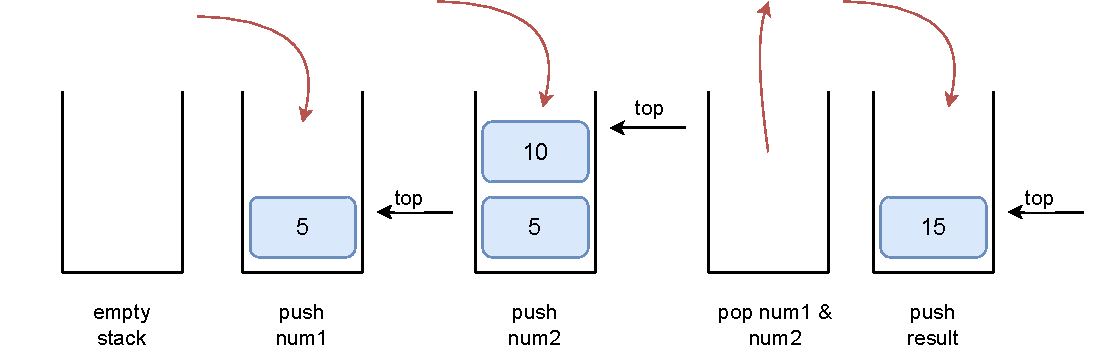
\includegraphics[width=1\linewidth]{images/wasm/stack_add_num_wasm.drawio.pdf}
  \caption{Visualization of how the stack is used to add two numbers in WebAssembly}
  \label{fig:stack_wasm_add_num}
\end{figure}
\section{WebAssembly Specification}
\label{sec:wasm-specification}

The \gls{WebAssembly} standard is developed by W3C Working Group (WG) and W3C Community Group (CG) \cite{webassemblycommunitygroup_2023_webassembly}. The WebAssembly specification document \cite{webassemblycommunitygroup_2023_webassembly} focuses on Wasm's core Instruction Set Architecture layer, defining the instruction set, binary encoding, validation, execution semantics, and textual representation. However, it does not specify how WebAssembly programs interact with the execution environment or how they are invoked within that environment \cite{webassemblycommunitygroup_2023_webassembly}.


The WebAssembly specification gets extended through proposals. From creating a proposal to fully integrating it into WebAssembly core specification, it must process through several phases. Each proposal follows this progression \cite{webassemblyw3c_2023_webassembly}:
\begin{itemize}
  \item \textbf{0. Pre-Proposal [Individual]}: An individual files an issue on the design repository to discuss the idea. The idea is then discussed and championed by one or more members. 
  The proposal's general interest is voted on by the Community Group to ensure its scope and viability.
  \item \textbf{1. Feature Proposal [CG]}: A repository is created, and the champion works on reaching broad consensus within the Community Group. The design is iterated upon, and prototype implementations may be created to demonstrate the feature's viability.
  \item \textbf{2. Feature Description Available [CG + WG]}: A precise and complete overview document is produced with a high level of consensus. Prototype implementations create a comprehensive 
  test suite, but updates to the reference interpreter and spec document aren't yet required.
  \item \textbf{3. Implementation Phase [CG + WG]}: WebAssembly runtimes implement the feature, the spec document is updated with full English prose and formalization, and the reference interpreter is updated with a complete implementation. Toolchains implement the feature, and any remaining open questions are resolved.
  \item \textbf{4. Standardize the Feature [WG]}: The feature is handed over to the Working Group, which discusses the feature, considers edge cases, and confirms consensus on its completion. 
  The Working Group periodically polls on the feature's "ship-worthiness." If only minor changes are needed, they are made; otherwise, the feature is sent back to the Community Group.
  \item \textbf{5. The Feature is Standardized [WG]}: Once consensus is reached among Working Group members that the feature is complete, editors merge the feature into the main branch of the primary spec repository of WebAssembly.
\end{itemize}

Throughout these phases, proposals are refined, adjusted, and tested to ensure their seamless integration with the existing WebAssembly specification. The following \autoref{tab:active-proposals} lists the active proposals and their current phase. The proposal repository \cite{webassemblywg_2023_webassembly} contains more information about each proposal, including the proposal's current phase, champion, and links to the proposal's repository and design document, furthermore, the repository also contains a list of all the proposals that have been merged into the WebAssembly core specification.

In the next three sections, we will elaborate two proposals that have been already integrated into the WebAssembly core specification and one that is still an active proposal. The first proposal is the multi-value return, which allows functions to return multiple values a common feature in modern programming languages. The second proposal is the reference types, which allows WebAssembly to handle complex data types \cite{couriol_2020_webassembly}. The third proposal is the \gls{WebAssembly} GC proposal, which depends on the reference types proposal and adds garbage collection to WebAssembly and thereby expanding the range of languages that can be compiled to WebAssembly. These proposals were especially chosen because they make the WebAssembly target more accessible to a broader range of languages and use cases.

\begin{table}[htbp]
  \centering
  \begin{tabular}{|ll|}
    \hline
    \multicolumn{2}{|c|}{\textbf{Phase 5 - The Feature is Standardized (WG)}}                                                                                                                              \\ \hline
    \multicolumn{1}{|c|}{\textbf{Proposal}}                              &\multicolumn{1}{c|}{\textbf{Champion}}                                                                                          \\ \hline
    \multicolumn{2}{|l|}{\textit{\begin{tabular}[c]{@{}l@{}}Currently, there is no active Phase 5 proposal\\ that has not been merged into the Wasm Core spec.\end{tabular}}}                              \\ \hline
    \multicolumn{2}{|c|}{\textbf{Phase 4 - Standardize the Feature (WG)}}                                                                                                                                  \\ \hline
    \multicolumn{1}{|l|}{Tail call}                                      & Andreas Rossberg                                                                                                                \\ \hline
    \multicolumn{1}{|l|}{Extended Constant Expressions}                  & Sam Clegg                                                                                                                       \\ \hline
    \multicolumn{2}{|c|}{\textbf{Phase 3 - Implementation Phase (CG + WG)}}                                                                                                                                \\ \hline
    \multicolumn{1}{|l|}{Multiple memories}                              & Andreas Rossberg                                                                                                                \\ \hline
    \multicolumn{1}{|l|}{Custom Annotation Syntax in the Text Format}    & Andreas Rossberg                                                                                                                \\ \hline
    \multicolumn{1}{|l|}{Memory64}                                       & Sam Clegg                                                                                                                       \\ \hline
    \multicolumn{1}{|l|}{Exception handling}                             & Heejin Ahn                                                                                                                      \\ \hline
    \multicolumn{1}{|l|}{Web Content Security Policy}                    & Francis McCabe                                                                                                                  \\ \hline
    \multicolumn{1}{|l|}{Branch Hinting}                                 & Yuri Iozzelli                                                                                                                   \\ \hline
    \multicolumn{1}{|l|}{Relaxed SIMD}                                   & Marat Dukhan \& Zhi An Ng                                                                                                       \\ \hline
    \multicolumn{1}{|l|}{Typed Function References}                      & Andreas Rossberg                                                                                                                \\ \hline
    \multicolumn{1}{|l|}{Garbage collection}                             & Andreas Rossberg                                                                                                                \\ \hline
    \multicolumn{1}{|l|}{Threads}                                        & Conrad Watt                                                                                                                     \\ \hline
    \multicolumn{1}{|l|}{JS Promise Integration}                         & Ross Tate \& Francis McCabe                                                                                                    \\ \hline
    \multicolumn{1}{|l|}{Type Reflection for WebAssembly JavaScript API} & Ilya Rezvov                                                                                                                     \\ \hline
    \multicolumn{2}{|c|}{\textbf{Phase 2 - Proposed Spec Text Available (CG + WG)}}                                                                                                                        \\ \hline
    \multicolumn{1}{|l|}{ECMAScript module integration}                  & Asumu Takikawa \& Ms2ger                                                                                                        \\ \hline
    \multicolumn{1}{|l|}{Relaxed dead code validation}                   & Conrad Watt and Ross Tate                                                                                                       \\ \hline
    \multicolumn{1}{|l|}{Numeric Values in WAT Data Segments}            & Ezzat Chamudi                                                                                                                   \\ \hline
    \multicolumn{1}{|l|}{Instrument and Tracing Technology}              & Richard Winterton                                                                                                               \\ \hline
    \multicolumn{2}{|c|}{\textbf{Phase 1 - Feature Proposal (CG)}}                                                                                                                                         \\ \hline
    \multicolumn{1}{|l|}{Type Imports}                                   & Andreas Rossberg                                                                                                                \\ \hline
    \multicolumn{1}{|l|}{Component Model}                                & Luke Wagner                                                                                                                     \\ \hline
    \multicolumn{1}{|l|}{WebAssembly C and C++ API}                      & Andreas Rossberg                                                                                                                \\ \hline
    \multicolumn{1}{|l|}{Extended Name Section}                          & Ashley Nelson                                                                                                                   \\ \hline
    \multicolumn{1}{|l|}{Flexible Vectors}                               & Petr Penzin                                                                                                                     \\ \hline
    \multicolumn{1}{|l|}{Call Tags}                                      & Ross Tate                                                                                                                       \\ \hline
    \multicolumn{1}{|l|}{Stack Switching}                                & Francis McCabe \& Sam Lindley                                                                                                   \\ \hline
    \multicolumn{1}{|l|}{Constant Time}                                  & \begin{tabular}[c]{@{}l@{}}Sunjay Cauligi, Garrett Gu, \\ John Renner, Hovav Shacham, \\ Deian Stefan \& Conrad Watt\end{tabular} \\ \hline
    \multicolumn{1}{|l|}{JS Customization for GC Objects}                & Asumu Takikawa                                                                                                                  \\ \hline
    \multicolumn{1}{|l|}{Memory control}                                 & Deepti Gandluri                                                                                                                 \\ \hline
    \multicolumn{1}{|l|}{Reference-Typed Strings}                        & Andy Wingo                                                                                                                      \\ \hline
    \multicolumn{1}{|l|}{Profiles}                                       & Andreas Rossberg                                                                                                                \\ \hline
    \multicolumn{2}{|c|}{\textbf{Phase 0 - Pre-Proposal (CG)}}                                                                                                                                                      \\ \hline
    \multicolumn{2}{|l|}{\textit{Currently, there is no active pre-proposal.}}                                                                                                                    \\ \hline
  \end{tabular}
  \caption{Active proposals in the WebAssembly CG and WG obtained from \cite{webassemblywg_2023_webassembly}}
  \label{tab:active-proposals}
\end{table}


\section{Multi-Value Return}
\label{sec:multi-value-return}

In modern programming languages that support tuples, like Kotlin, Rust or Python, developers can effortlessly bundle several values into a single structure for returning from a function. 
Simple tasks, such as switching a pair of values or sorting an array, become challenging since they must be performed within the linear memory block. 
Some arithmetic functions, including modular operations and carry bits, can also yield multiple values.

Aside from functions that return tuples or multiple values, another limitation in the \hbox{WebAssembly} MVP was that loops and conditional blocks, in the code base cannot process or return more than one result \cite{sletten_2021_webassembly}. 
It would be equally intriguing to exchange values, perform arithmetic with overflow, or receive a multi-value tuple response in these scenarios as well. 
Furthermore, compilers are no longer required to jump through hoops when generating multiple stack values for core WebAssembly. This results in smaller generated bytecode and consequently, faster loading times and brings an extension type which is common in some programming languages like Rust or Python. Currently, the proposal has been already integrated into the WebAssembly core specification \cite{webassemblywg_2023_webassembly}. 

This proposal introduces a new type of arithmetic instruction "i32.divmod" \cite{fitzgerald_2019_multivalue, webassemblycommunitygroup_2023_webassembly} which takes a numerator and divisor and returns the quotient and remainder. Moreover, it enables multiple values to stay on the stack without needing to be copied into linear memory.

The most effective way to demonstrate the proposal is by presenting a straightforward example. In example \ref{code:multi-values}, we have a WAT file with an exported function called "reverseSub" that subtracts the second parameter from the first one and returns the result. 

Firstly, we define a module that contains two functions. The first one is an internal function called "swap" that takes two i32 (32-bit integer) parameters and returns them in reverse order. The second function is the one that we want to export and is called "reverseSub". It takes two 32 bit integer (i32) parameters and returns an integer (i32) result value. An exported function, means it will be accessible outside the WebAssembly module. Notice that "local.get 0" and "local.get 1" instructions are used to get the first and second parameters respectively. The "call \$swap" instruction calls the "swap" function and passes the two parameters to it. Finally, the "i32.sub" instruction \cite{webassemblycommunitygroup_2023_webassembly} subtracts the second parameter from the first one and returns the result.

\begin{lstlisting}[frame=lines, style=Wasm, caption={A Wasm module with a reverse subtraction function returning multiple values}, showstringspaces=false, captionpos=b, label=code:multi-values]
(module ;; reverseSub.wat
  (func $swap (param i32 i32) (result i32 i32)
    local.get 1
    local.get 0)

  (func (export "reverseSub") (param i32 i32) (result i32)
    local.get 0
    local.get 1
    call $swap
    i32.sub)
)
\end{lstlisting}

\section{Reference Types}
\label{sec:reference-types}

Before the introduction of reference types, WebAssembly only supported four primitive value types \cite{webassemblycommunitygroup_2023_webassembly}: 32-bit integers, 64-bit integers, 32-bit floating-points, and 64-bit floating-point numbers. With the introduction of reference types, WebAssembly capabilities are extended to include garbage-collected references. This will enable other proposals \cite{couriol_2020_webassembly} such as the garbage collection proposal, type import proposal (see \autoref{tab:active-proposals}) and more to utilize reference types without the need for glue code or dangerous workarounds. 

For instance, as Nick Fitzgerald noted in his publication \cite{fitzgerald_2020_webassembly}, the host stores objects in a side table and passes the indexes to the Wasm module. The Wasm module then uses these indexes to retrieve the objects from the side table. The usage of side tables requires glue code and is error-prone. Moreover, the glue code needs to be written in the host's language, making the Wasm module less portable.

The reference types proposal makes it possible for the host to specify and pass opaque handles to WebAssembly modules. These handles can be used to reference objects in the host environment, such as DOM nodes of a web page, a file handle or even open connection to a database. 

The reference types proposal brings three new features:
\begin{itemize}
    \item Makes it possible to have a \texttt{externref} type which is a opaque and unforgable reference to a object in the host environment.
    \item Makes it possible to store \texttt{externref} values in Wasm tables.
    \item Makes it possible to manipulate table entities with the help of new instructions.
\end{itemize}

As mentioned in the first bullet point, \texttt{externref} has two beneficial properties that fits the sandbox model of WebAssembly:
\begin{itemize}
    \item \textbf{Opaque}: The \texttt{externref} type is opaque, meaning that the reference does not reveal any significant information about the object it is referencing or the memory layout of the host environment.
    \item \textbf{Unforgable}: The \texttt{externref} type is unforgable, meaning it can either return a null reference or the same reference that was passed to the Wasm module. This prevents the Wasm module from creating new references to objects in the host environment. It makes it impossible to forge the reference. 
\end{itemize}

%TODO: Add example of how to use reference types

\section{Garbage Collection Proposal (Wasm GC)}
\label{sec:gc-proposals}

The garbage collection proposal \cite{webassemblycommunity_2023_gc} is currently under active development. This is one of the most anticipated proposals since it will enable developers to use managed-memory languages such as Kotlin, Java, Dart and many more to the WebAssembly ecosystem. 

Prior to this proposal, managed-memory languages have to ship and instantiate their own garbage collector every time the app loads, thus, increasing the \gls{WebAssembly} module size and increasing the startup time, even when every standard browser already has a garbage collector. \autoref{fig:wasm-gc-1} illustrates this problem, marked as "\#1 bloat problem", very well. Another issue is the fact that developers need to know how large the heap is going to be, to avoid running out of memory. A typical thing todo is to allocate a large amount of memory and hope that it is enough. This architecture treats the Wasm module as a separate entity from the host environment, even though it might reference objects in the host environment. This brings us to the next issue, marked as "\#2 split brain problem", there is no guarantee that the references in the JavaScript Heap are still valid, because there is no way to inform the garbage collector that the Wasm module is no longer using the reference or vice versa. This is a problem because the garbage collector might free the memory that the reference is pointing to, which will result in a dangling pointer. 

Even supposing that developers keep the references on the Wasm module side, there is still the possibility that we might need the JavaScript heap, due to the fact that the Wasm module might need to call Web APIs. Web APIs accept only JavaScript objects that live on the JavaScript heap. 
%
\begin{figure}[htbp]
  \centering
      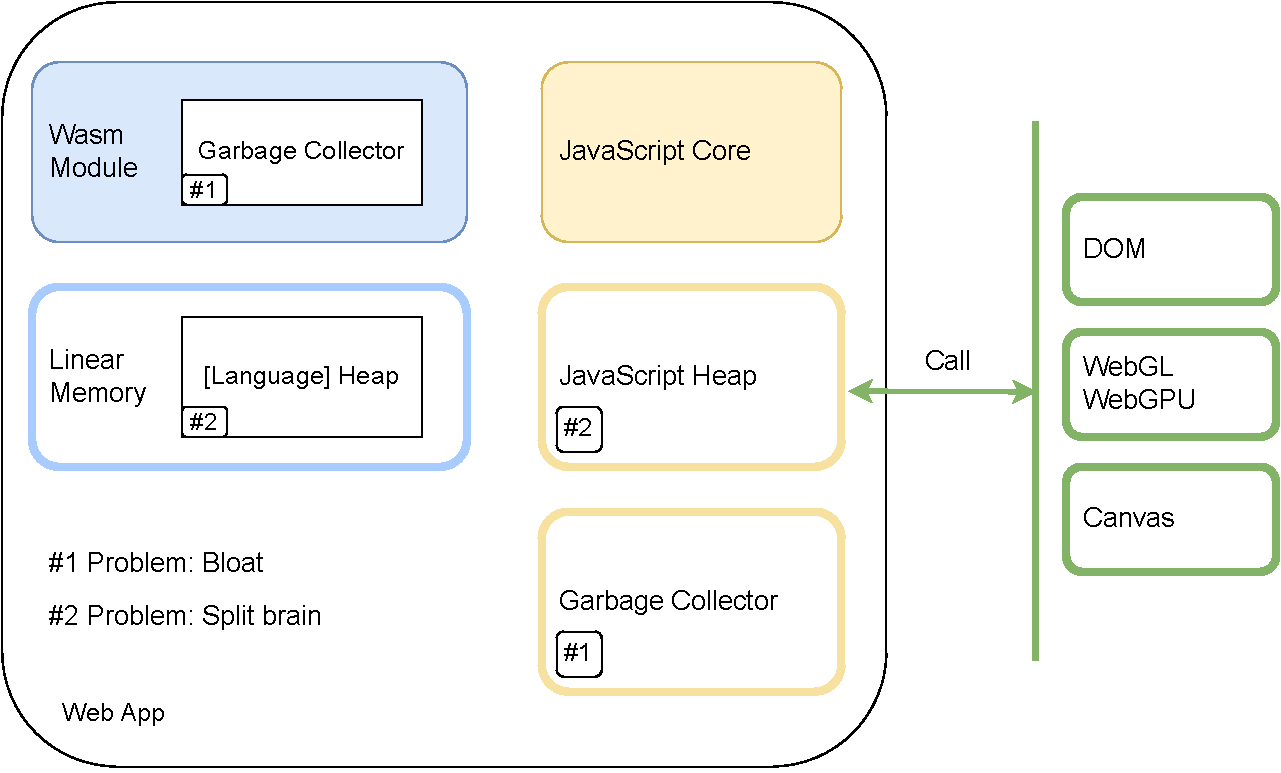
\includegraphics[width=1\linewidth]{images/wasm/wasm_gc_1.drawio.pdf}
  \caption{Wasm module without garbage collection proposal based on \cite{sekhar_2023_mobile}}
  \label{fig:wasm-gc-1}
\end{figure}
%
The Wasm GC proposal makes it possible to have a joint heap between JavaScript and WebAssembly GC code. This way the managed-memory code can allocate objects on the joint heap and when the JavaScript garbage collector runs, it will also collect the WebAssembly GC memory, because they are using the same heap memory (see \autoref{fig:wasm-gc-2}). Furthermore, depending on the runtime implementation, the runtime can return the unused memory back to the operating system to ensure the efficiency and responsiveness of the application \cite{sekhar_2023_mobile}. 

This means that the Wasm module doesn't have to include it's own garbage collector, which will reduce the Wasm module size and startup time. Moreover, the Wasm module can easily grow or shrink the memory based on consumption. 

To summarize, according to Vivek Sekhar in Wasm I/O 2023 conference, the garbage collection proposal brings the following three benefits \cite{sekhar_2023_mobile}:
%
\begin{itemize}
  \item \textbf{Smaller binaries for managed-memory languages}: Languages with dedicated garbage collectors no longer need to ship the garbage collector with the runtime. The hosts garbage collector can be used to garbage collect JavaScript and WebAssembly memory.
  \item \textbf{Enhanced interoperability with JavaScript code and Web APIs}: Wasm modules can directly access Web APIs, such as DOM, WebGL, Canvas, and more. Furthermore, objects can be passed to the JavaScript code, eliminating the need to copy objects between JavaScript and WebAssembly memories.
  \item \textbf{Resizable memory footprint}: The memory footprint can adjust to the usage and therefore additional memory can be allocated to WasmGC module. Unused memory can be returned to the host environment.
\end{itemize}
%
\begin{figure}[htbp]
  \centering
      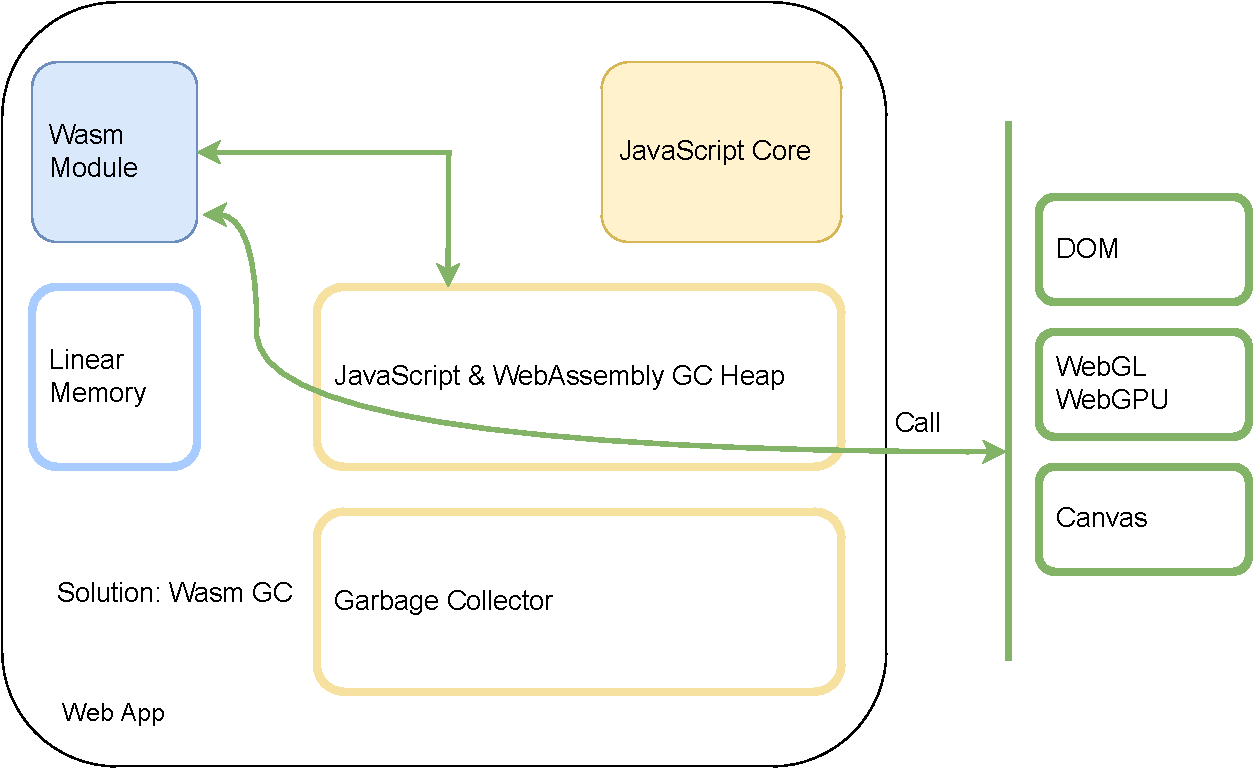
\includegraphics[width=1\linewidth]{images/wasm/wasm_gc_2.drawio.pdf}
  \caption{Wasm module with garbage collection proposal based on \cite{sekhar_2023_mobile}}
  \label{fig:wasm-gc-2}
\end{figure}
%
Even though the garbage collection proposal is still under active development, the Kotlin team has already rolled out an experimental compiler based on the proposal \cite{kotlin_2023_kotlin}.

\section{WebAssembly System Interface (WASI)}
\label{sec:wasi}
While WebAssembly is primarily designed for efficient operation on the web, as previously mentioned, it avoids making web-specific assumptions or integrating web-specific features. 
The core WebAssembly language remains independent of its surrounding environment and interacts with external elements exclusively through APIs. When operating on the web, it seamlessly utilizes existing web APIs provided by browsers. However, outside the browser environment, there is currently no standardized set of APIs for developing WebAssembly programs. This lack of standardization poses challenges in creating truly portable WebAssembly programs for non-web applications.

The WebAssembly System Interface (abbriveated as WASI) in short is a standard interface for WebAssembly modules to interact with their host environments, such as operating systems, without being tied to any specific host. This allows WebAssembly modules to be executed securely and portably across a wide range of environments. 

The aim of WASI is to be a highly modular set of system interfaces, which includes both low-level and high-level interfaces like \gls{POSIX} functions, neural networks, cryptography and so on. 
It is anticipated that more high-level APIs will be incorporated in the future depending on the priorities of the ecosystem. These interfaces must adhere to capability-based security principles to preserve the sandbox's integrity. Additionally, the interfaces should be portable across major operating systems, although system-specific interfaces may be acceptable for certain 
narrow use cases.

According to Dan Gohman's proposed roadmap, the development of WASI is set to progress through Preview1, Preview2, and Preview3. 
Currently, the community is actively working on Preview2, however, each stage will be backward compatible. 

\begin{figure}[H]
	\centering
		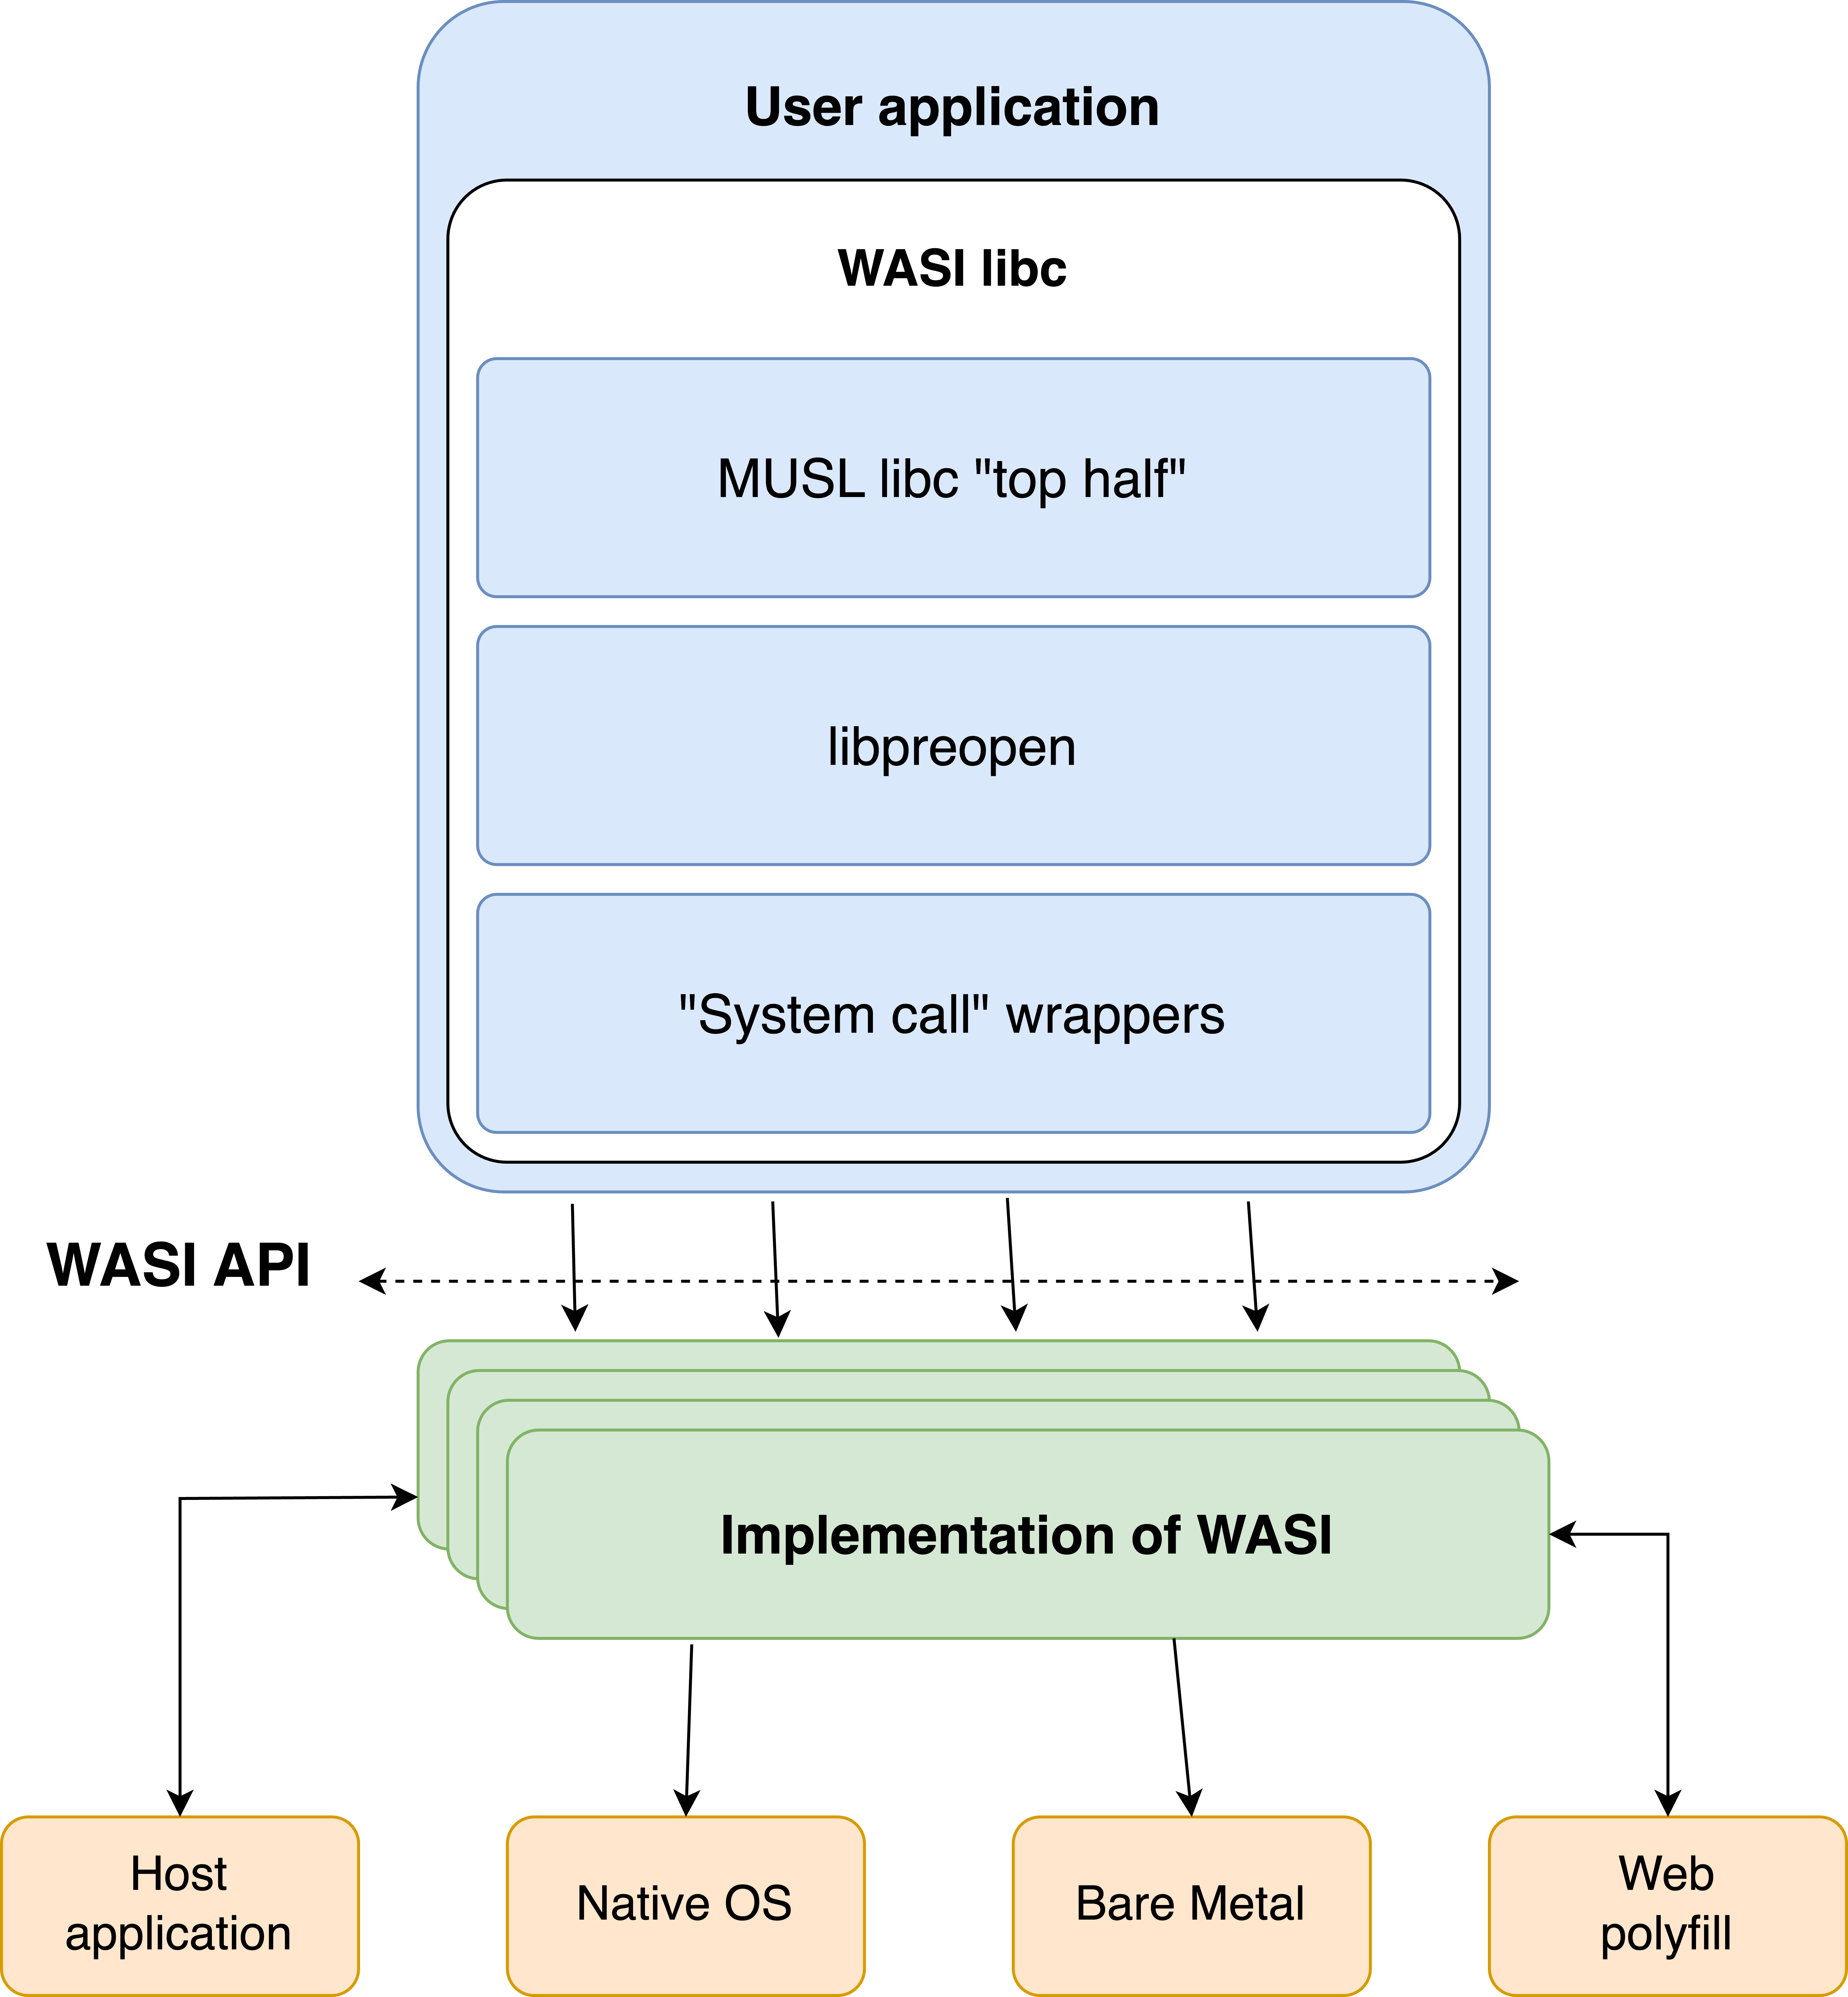
\includegraphics[width=130mm,scale=0.8]{images/wasm/WASI_Architecture.png}
	\caption{WASI Architecture}
	\label{fig:wasi-architecture}
\end{figure}

\subsection{WASI as Emscripten replacement?}
The first toolchain that enabled C, C++, or any other language with \gls{LLVM} support to be compiled into WebAssembly was Emscripten. Essentially, Emscripten can compile almost any portable C or C++ codebase into WebAssembly, encompassing high-performance games requiring graphics rendering, sound playback, and file loading and processing, as well as application frameworks like Qt. Emscripten has been utilized to convert numerous applications like Unreal Engine 4 and the Unity engine, into WebAssembly \cite{emscriptencommunity_2023_emscripten}. 

To achieve this, Emscripten implemented the \gls{POSIX} OS system interface on the web. 
As a result, developers are able to use the functions available in the C standard library (\gls{libc}). 
Emscripten accomplished this by creating its own implementation of libc, which was divided into two parts. One part was compiled into the WebAssembly module, while the other part was implemented in \gls{JS glue code}. 
The JS glue would subsequently communicate with the browser, which would in turn communicate with the Kernel and the OS.

\begin{figure}[H]
    \centering
        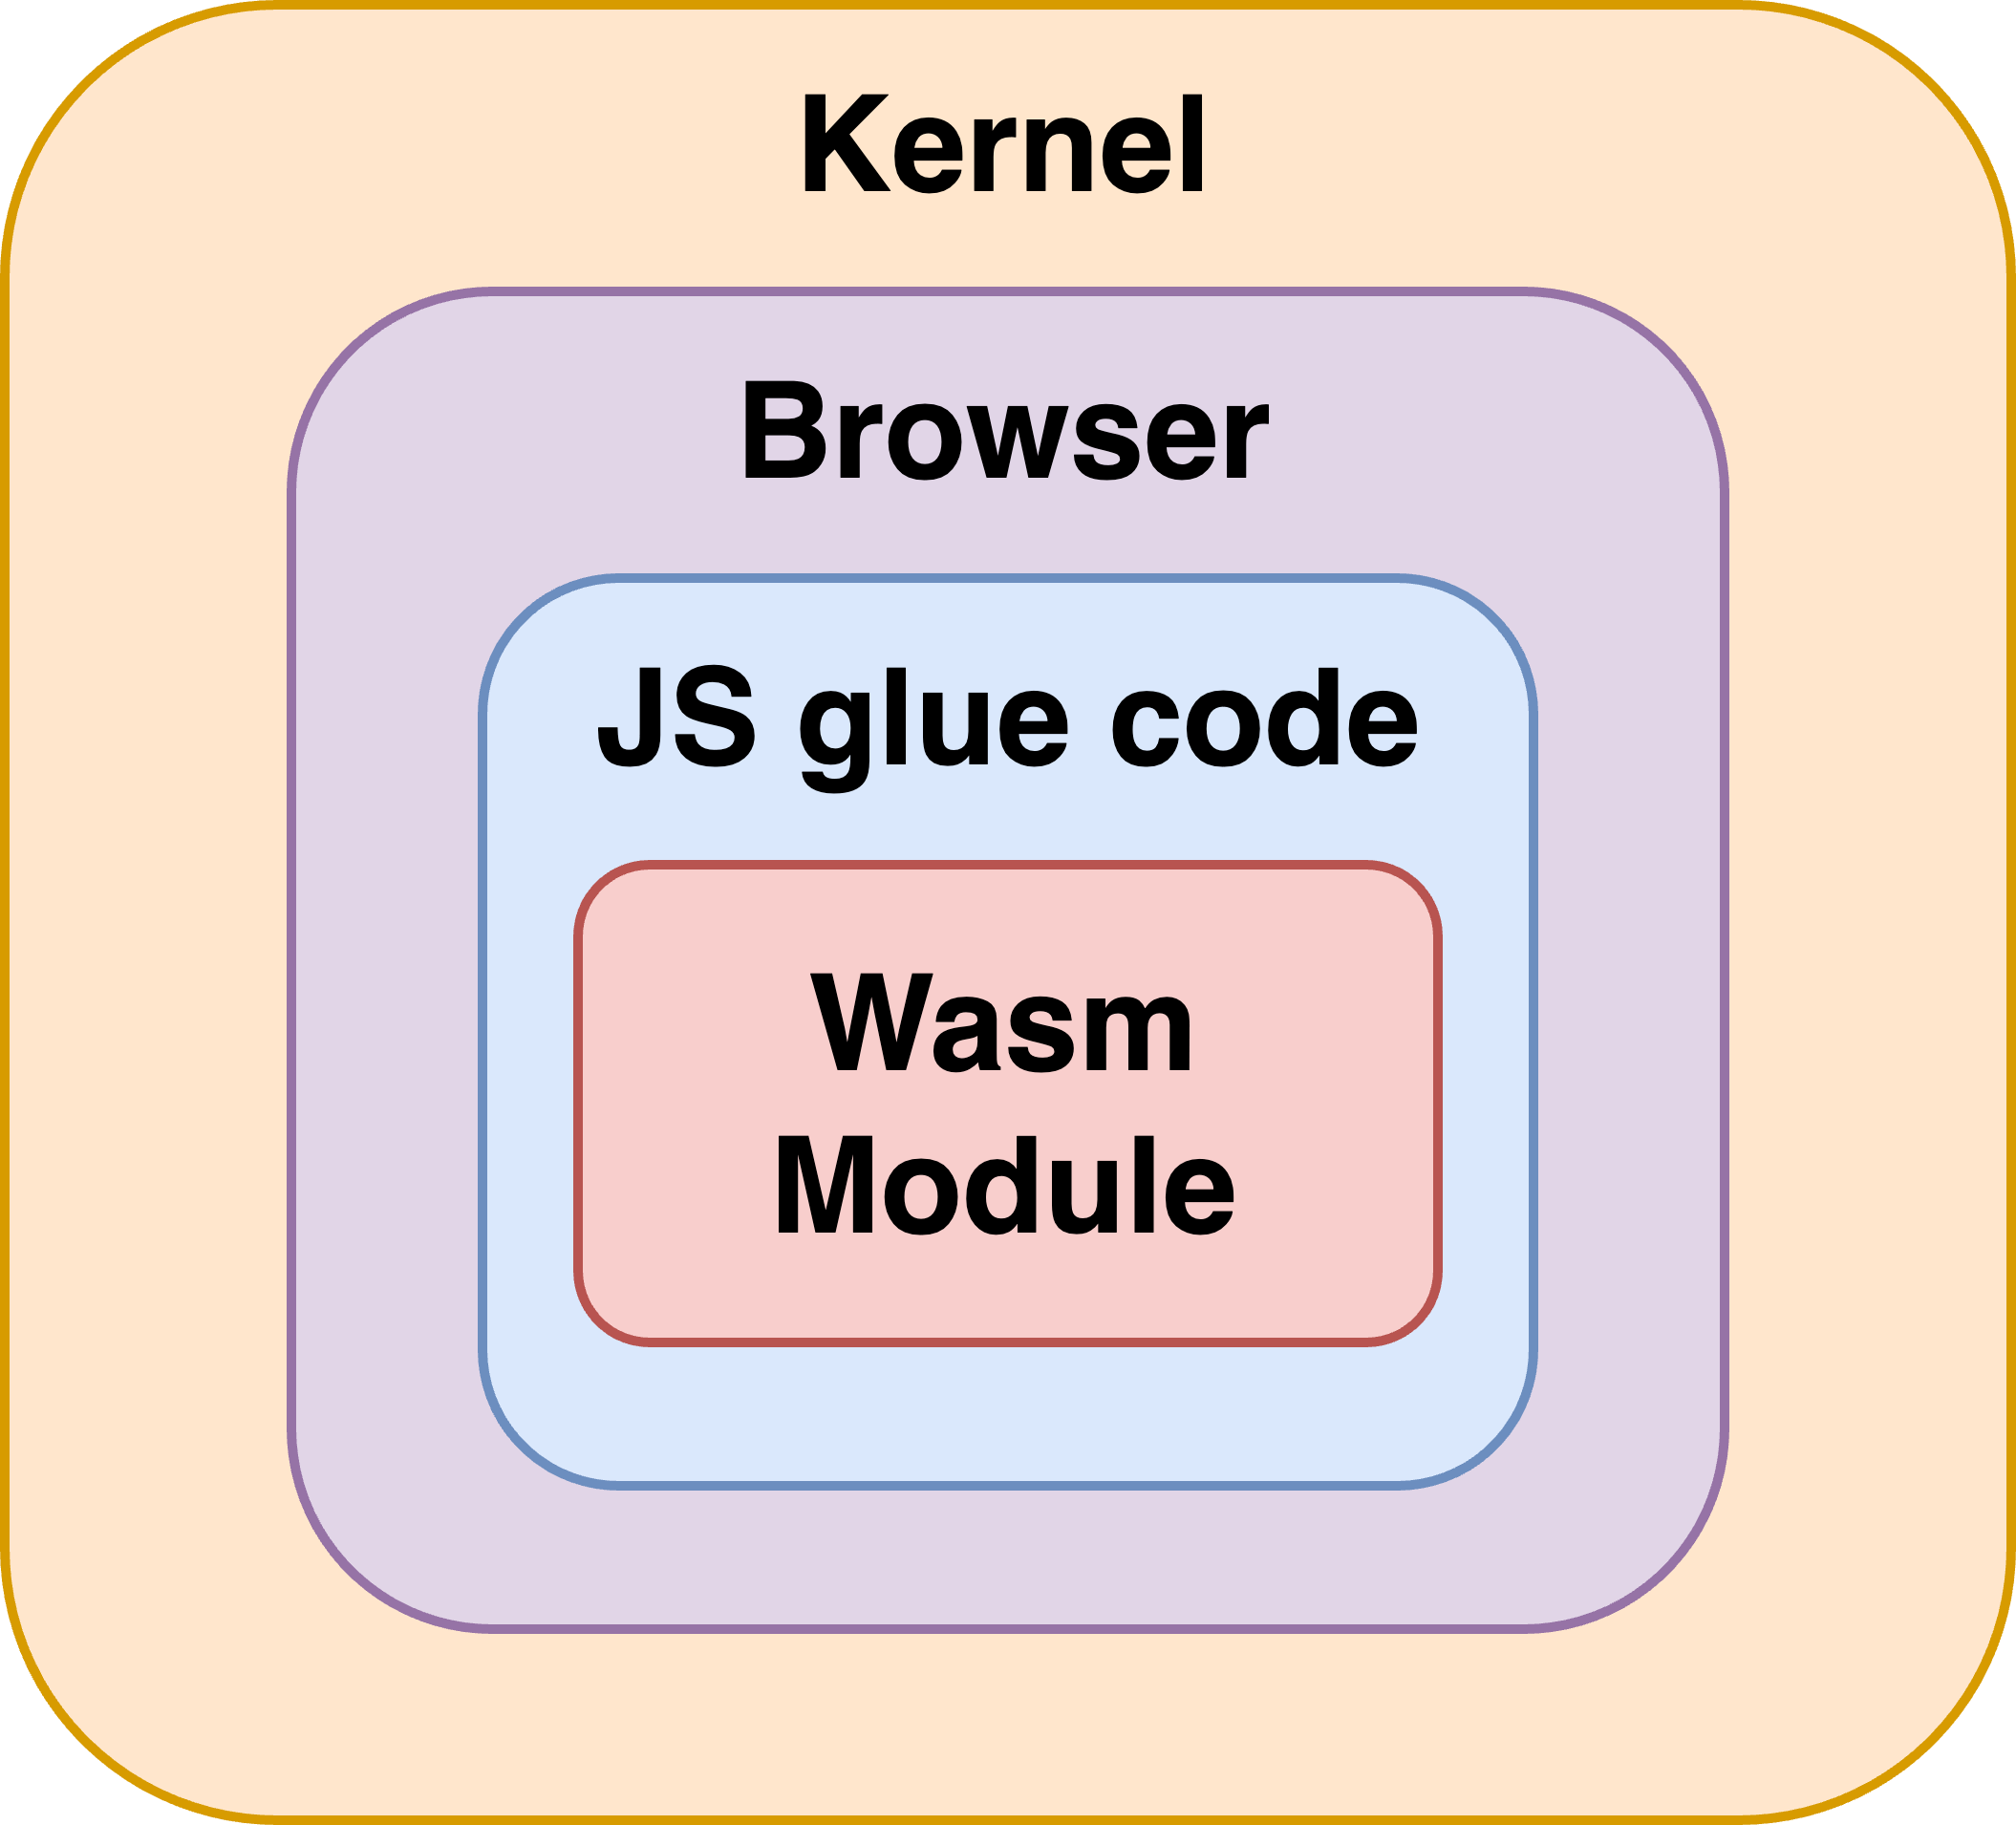
\includegraphics[width=0.6\linewidth]{images/wasm/Emscripten.png}
    \caption{Structure of Emscripten compiled Wasm module}
    \label{fig:emscripten}
\end{figure}

When users began to seek ways of running WebAssembly outside of a browser environment, the first approach was to enable the execution of Emscripten-compiled code on the corresponding environment.
To achieve this, the runtimes had to develop their own implementations of the functions in the JS glue code. However, this presented a challenge as the interface provided by the JS glue code was not intended to be a standard or public-facing interface. 
It was designed to serve a specific purpose, and creating a portable interface was not part of its intended design. The above figure \ref{fig:emscripten} shows the connection between the browser, the glue code and the Wasm module. 

Emscripten aims to improve the standard by using WASI APIs as extensively as possible in order to minimize unnecessary API differences. As previously stated, Emscripten code accesses Web APIs indirectly via JavaScript on the web. By making the JavaScript API resemble WASI, an unnecessary API difference can be eliminated, allowing the same binary to run on a server as well. In simpler terms, if a Wasm application wants to log information, it must call into JavaScript, following a process similar to this:

\verb|wasm => function musl_writev(...) { ... console.log(...) ... }|

"musl\_writev" represents an implementation of the Linux syscall interface utilized by "musl libc" to write data to a file descriptor, ultimately leading to a call to console.log with the appropriate data. The Wasm module imports and invokes "musl\_writev", thereby defining an ABI between the JavaScript and Wasm components. This ABI is arbitrary, by changing the existing ABI with one that aligns with WASI, the following can be achieved:

\verb|wasm => function __wasi_fd_write(...) { ... console.log(...) ... }|

% X 1. die API zu einem gewissen grad vereinheitlichen kann
% 2. es gibt dinge die emscripten machen kann aber wasi nicht macht
% 3. es macht vielleicht auch sinn eine api für web eine api für server und andere api's für plugins zu haben

%According to \cite{zakai_2019_outside} 

\subsection{WASI Portability}
\label{subsec:wasi-portability}

WebAssembly by design is a portable format, as mentioned before, the core specification does not make any platform specific assumptions. 
The first system API which the WASI community has been working on is the \gls{POSIX} API. 
It involves essential functionalities like file operations, processes, threads, 
shared memory, networking, regular expressions and so on. WASI will consist of a collection of low level and high level APIs, which aim to be as portable as possible. 

Figure \ref{fig:wasi-portability} illustrates that a source code can be compiled with different versions of libc to target various platforms. However, in the case of WASI, the same source code can be compiled into a portable binary that targets a virtual host platform called "wasm32-unknown-wasi". 
This target comprises three parts: the underlying architecture "wasm32", the vendor (which usually specifies the platform or hardware vendor; in this case, it is "unknown"), and the operating system ("wasi").

Comparing the left and right sides of the figure, we can observe that the Wasm binary runs on a WASI runtime, also known as a WASI engine. The implementation details of the underlying OS are abstracted away from the Wasm binary targeting WASI. For instance, suppose a small C program that opens a file, reads its contents, and prints them to the console. In that case, on a Linux system, the program would call the "open" syscall. 
However, on WASI, the program would call the "wasi\_fd\_open" function, which is part of the WASI API. 
The WASI module expects the engine to create a file descriptor and return it to the module, which it can then use to read the file contents.

\begin{figure}[H]
    \centering
        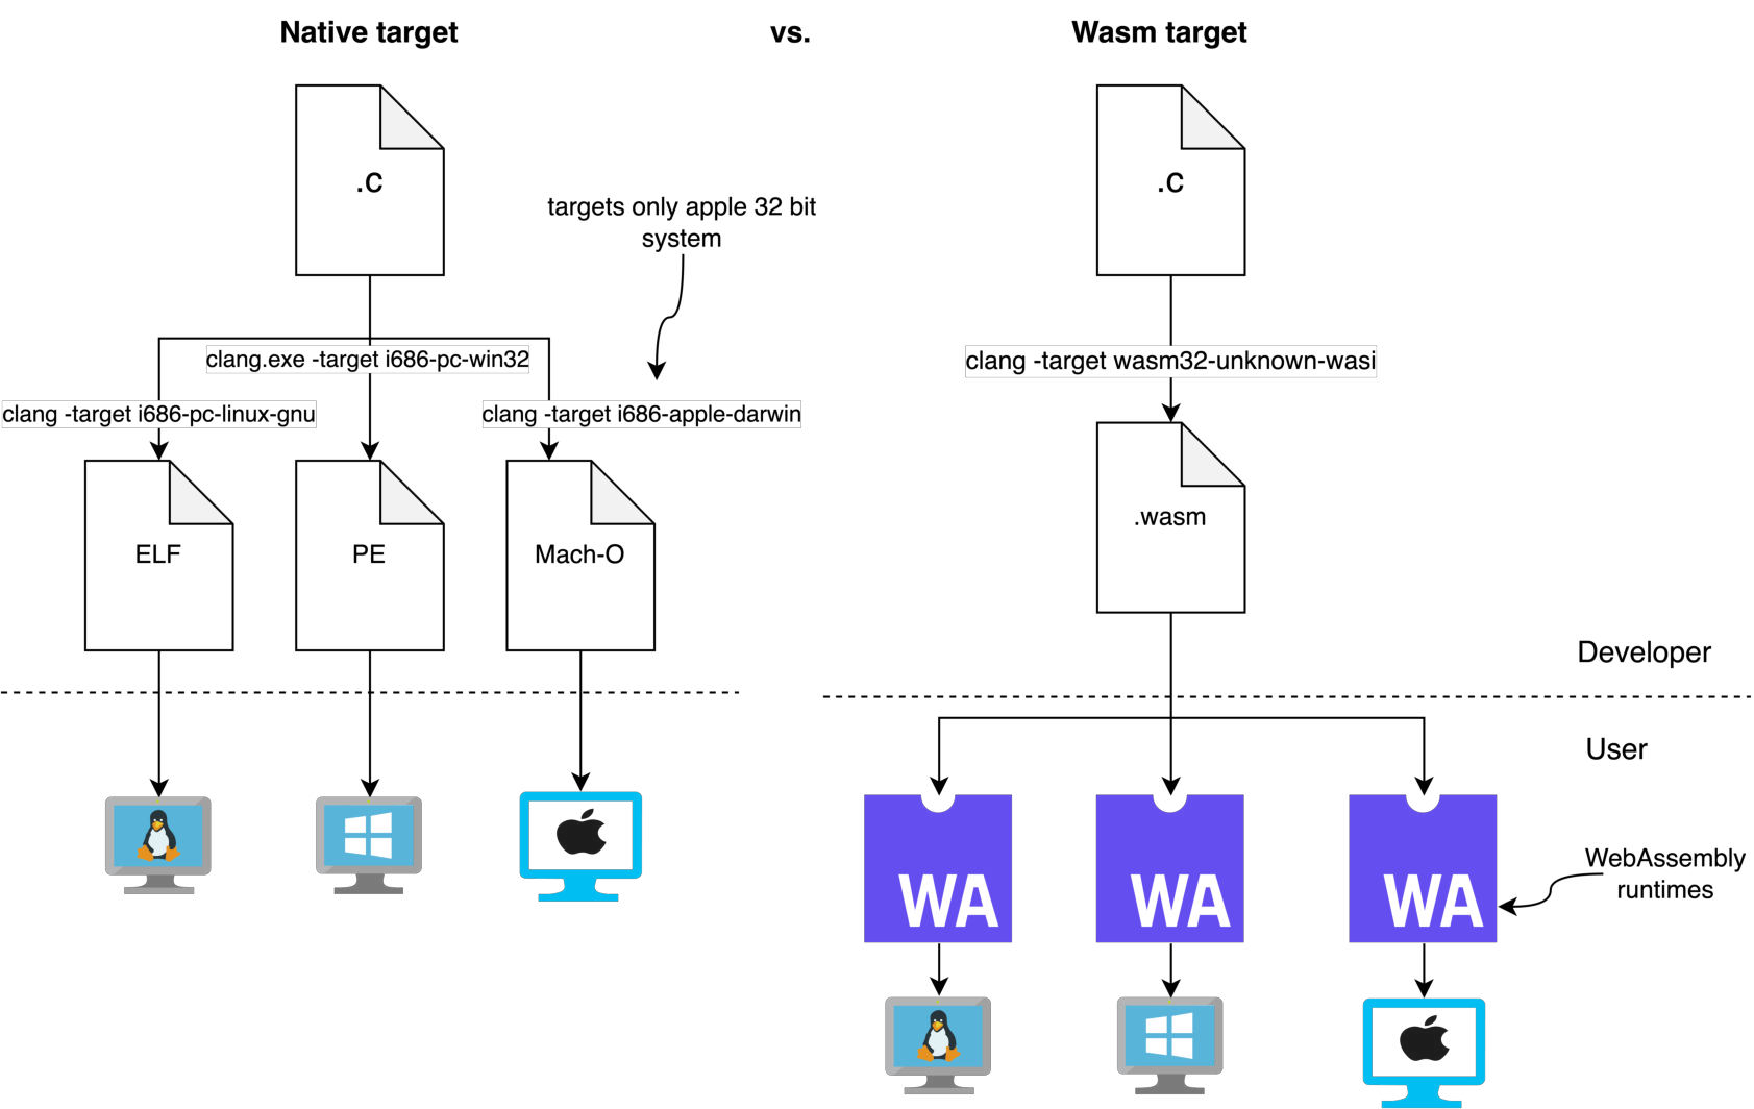
\includegraphics[width=1\linewidth]{images/wasm/WASI_PORTABILITY.pdf}
    \caption{WASI portability model redrawn from \cite{clark_2019_standardising}}
    \label{fig:wasi-portability}
\end{figure}

Aside from the information provided in Figure \ref{fig:wasi-portability}, it should be noted that because of WASI's portability, the modules are not confined to a particular host platform. They have the flexibility to be integrated into an application, function as a plugin, or run as a serverless function in the cloud, as referenced in \cite{clark_2022_wasmtime}, as long as the host runtime supports the required APIs.

\subsection{WASI Security Model}
\label{subsec:wasi-security-model}

An essential aspect of any system is the security model implemented to ensure the integrity and confidentiality of data and resources. When a code segment requests the operating system (OS) to perform input or output operations, the OS must ascertain whether the action is secure and permissible.

Operating systems generally employ an access control mechanism based on ownership and group associations to manage security. For instance, consider a scenario where a program seeks permission from the OS to access a specific file. Each user possesses a unique set of files they are authorized to access. In Unix systems, for example, the ownership of a file can be assigned to three classes of users: user, group, and others.

Upon initiating the program, it operates on behalf of the respective user. Consequently, if the user has access to the file—either as the owner or as a member of a group with access rights—the program inherits the same privileges. This approach to security helps maintain a robust and reliable system that adheres to the principles of access control and resource protection.

This approach was effective in multi-user systems where administrators controlled software installation, and the primary threat was unauthorized user access. However, in modern single-user systems, the main risk comes from the code that the user runs, which often includes third-party code of unknown trustworthiness. This raises the risk of a supply chain attack, particularly when new maintainers take over open-source libraries, as their unrestricted access could enable them to write code that compromises system security by accessing files or sending them over the network \cite{clark_2019_standardising}.

 % explain supply chain attack

The security aspect of WASI is vital to the universal nature of WebAssembly. The WASI standard was built on a capabilities-based security model, which means the host has to explicitly permit capabilities such as file system access and establishing network sockets. As a result, a WASI module cannot run arbitrary code with direct access to memory.

In the context of serverless computing, for instance, a cloud provider may allow or deny access to specific functions, thus implementing security policies on a per-function basis. However, this level of granularity may not be sufficient. Since WebAssembly does not employ virtualization, all modules share common resources, such as the file system. As a result, the cloud provider may want to permit serverless functions to temporarily cache data in a specific "/tmp/<unique-id>/" directory while forbidding access to confidential files like "/etc/passwd". This is where WASI incorporates concepts from capability-based security.


\chapter{Runtimes}
\label{chap:runtimes}

Table \ref{tab:runtime-overview}

(Why different runtimes? Motivation?)

\begin{table}[htbp]
  \small
  \begin{tabular}{|c|c|c|c|c|c|}
    \hline
    \textbf{Runtime} & \textbf{Embeddable langs.}                                                                                               & \textbf{Architecture}                                                                                                & \textbf{Compiler}                                                         & \textbf{Compilation}                                        & \textbf{Platform}                                                                             \\ \hline
    Wasmtime         & Rust, Python                                                                                                                & \begin{tabular}[c]{@{}c@{}}x86, \\ x86\_64, \\ ARM\end{tabular}                                                      & \begin{tabular}[c]{@{}c@{}}Cranelift, \\ LLVM\end{tabular}                & JIT, AoT                                                    & \begin{tabular}[c]{@{}c@{}}Windows, \\ Linux, \\ Mac OS\end{tabular}                          \\ \hline
    Wasmer           & Rust, C++                                                                                                                   & \begin{tabular}[c]{@{}c@{}}x86, \\ x86\_64, \\ ARM\end{tabular}                                                      & \begin{tabular}[c]{@{}c@{}}Cranelift, \\ LLVM, \\ Singlepass\end{tabular} & JIT, AoT                                                    & \begin{tabular}[c]{@{}c@{}}Windows, \\ Linux, \\ Mac OS, \\ Free BSD, \\ Android\end{tabular} \\ \hline
    Wasm3            & \begin{tabular}[c]{@{}c@{}}Python3, Rust, \\ GoLang, \\ Zig, Perl, Swift, \\ C\# .NET\end{tabular}                          & \begin{tabular}[c]{@{}c@{}}x86, \\ x86\_64, \\ ARM, \\ RISC-V, \\ PowerPC, \\ MIPS, \\ Xtensa, \\ ARC32\end{tabular} & Custom                                                                    & Interpreter                                                 & \begin{tabular}[c]{@{}c@{}}Windows, \\ Linux, \\ Mac OS, \\ Free BSD, \\ Android\end{tabular} \\ \hline
    WasmEdge         & \begin{tabular}[c]{@{}c@{}}Solidity, Rust, \\ C++, TinyGo, \\ JavaScript, Python, \\ Grain, Swift,\\ Zig, Ruby\end{tabular} & \begin{tabular}[c]{@{}c@{}}x86, \\ x86\_64, \\ ARM\end{tabular}                                                      & LLVM                                                                      & \begin{tabular}[c]{@{}c@{}}Interpreter, \\ AoT\end{tabular} & \begin{tabular}[c]{@{}c@{}}Windows, \\ Linux, \\ Mac OS, \\ Android\end{tabular}              \\ \hline
  \end{tabular}
  \caption{WebAssembly Runtimes overview based on \cite{akinyemi_2023_awesome}}
  \label{tab:runtime-overview}
\end{table}
    

\section{Serverless Requirements}
\label{sec:serverless-requirements}

The following summary of requirements should be met by an ideal serverless runtime, therefore, we will use them as a guideline to evaluate the different runtimes.

A serverless runtime should be able to:

\begin{enumerate}
	\item Ensure security and isolation between functions.
	\item Have a small footprint to reduce the startup time of functions, therefore, a small memory footprint and also fast startup time. 
	\item Integrate effortlessly with existing frameworks. 
	\item Support multiple programming languages but not less to the traditional serverless platforms. 
	\item Execute functions with a speed comparable to native speed.
	\item Have the capability to run on various instruction set architectures, including but not limited to \texttt{x86\_64} and \texttt{arm}.
	\item Handle large amount of I/O operations concurrently.
\end{enumerate}

\section{Evaluation of features}
\label{sec:evaluation-of-features}

\section{Execution Models}
\label{sec:execution-models}

\subsection{JIT - Just In Time Compilation}
\label{sec:jit}

\subsection{Interpreter}
\label{sec:interpreter}

\subsection{WASM to native compilation}
\label{sec:wasm-to-native}

\subsection{AOT - Ahead Of Time Compilation}
\label{sec:aot}


\subsection{Wasm Snapshots (Wizer)}
\label{sec:wizer}

As noted earlier, for serverless functions, having a fast startup time is crucial. 
Thus, techniques that can remove the repetitive initialization step from the critical 
path are highly beneficial. Wizer is a tool that can create a snapshot of an already 
initialized WebAssembly module. The snapshot is a pre-initialized Wasm module that should start 
faster without sacrificing any security or portability. 

As shown in Figure \ref{fig:wizer}, a program needs to go through four phases before it can be executed. 
The steps can be divided into two sections - the time of the developer spends to build and upload the program and the time of the user waiting for the program to become interactive on each request. The user experience can be enhanced by reducing the time spent in the second section. 

\begin{figure}[H]
	\centering
	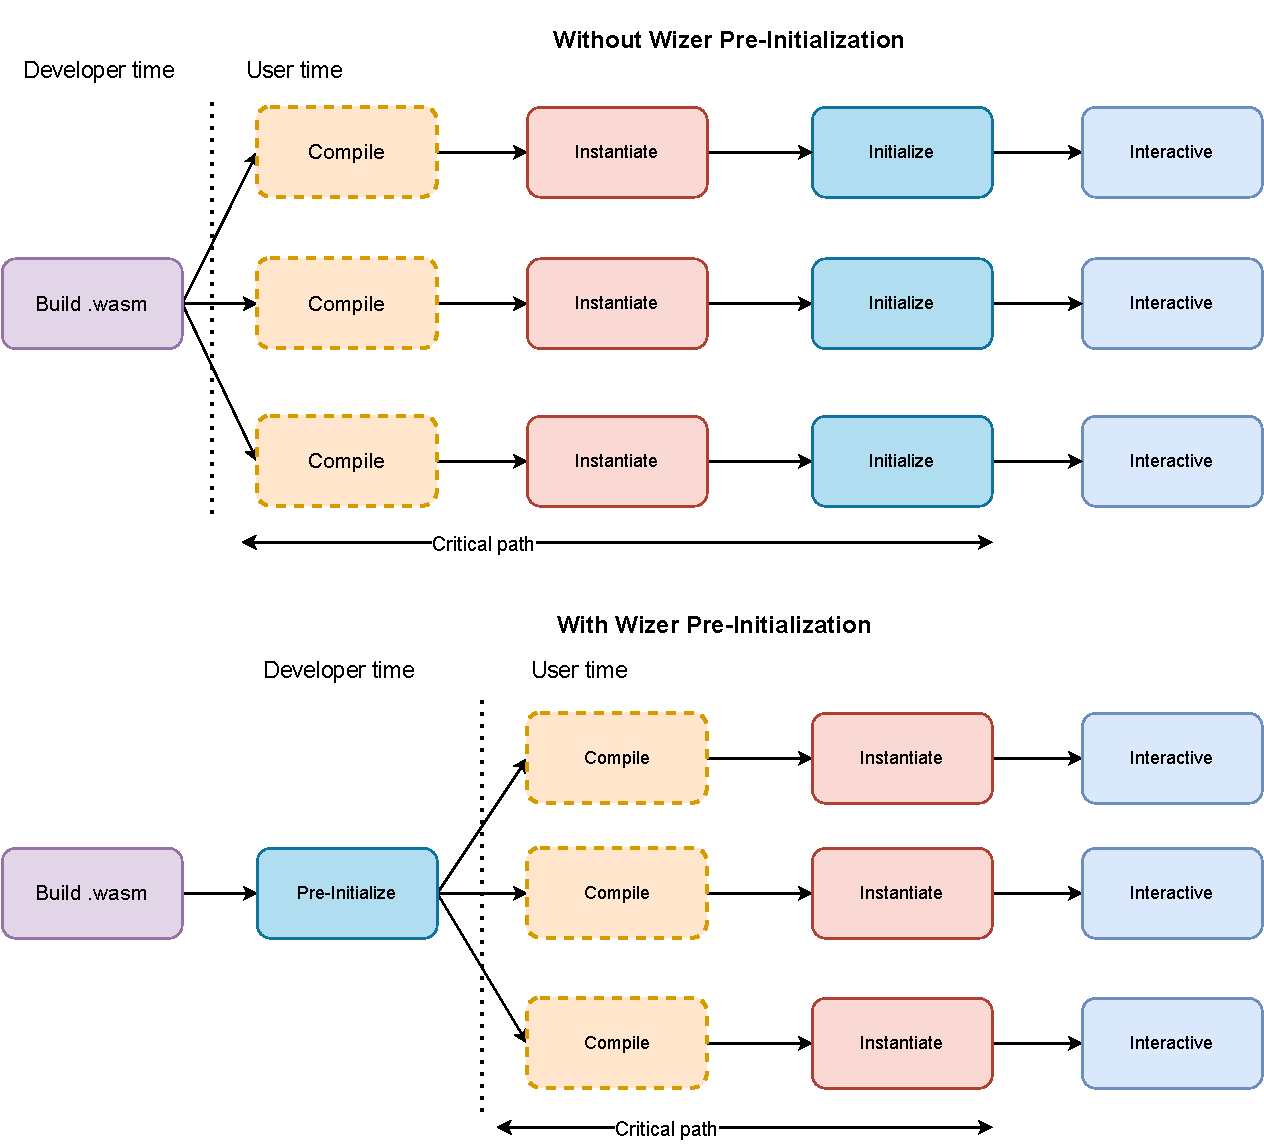
\includegraphics[width=0.8\linewidth]{images/runtimes/Wizer.drawio.pdf}
	\caption{Overview of Pre-initialization vs. Non Pre-initialization, based on \cite{fitzgerald_2021_hit}}
	\label{fig:wizer}
\end{figure}

Wizer creates a pre-initialized snapshot through these four phases \cite{fitzgerald_2021_hit}:
\begin{enumerate}
	\item Instrument: The first phase, known as the instrumentation phase, aims to export the internal state of the Wasm module so that Wizer can read it during the snapshot phase.
	\item Initialize: In the second phase, Wizer uses the Wasmtime runtime to compile and initialize the Wasm module. It then calls the exported "wizer.initialize" function.
	\item Snapshot: The third phase is the snapshot phase, in which Wizer reads the exports created in the first phase and generates the snapshot structure.
	\item Rewrite: The final phase is the rewrite phase. Wizer takes the initial Wasm module and the snapshot to create a new Wasm module. It removes the start section, as the snapshot has already executed the initializations, and updates each memory's minimum size to the size of the snapshot memories, as they may have grown during the initialization phase.
\end{enumerate}


\subsubsection{Wizer benchmarks}
\label{sec:wizer-benchmarks}

Initial benchmarks indicate that Wizer can provide between 1.35 and 6.00 times faster instantiation and initialization, depending on the specific workload. Running the benchmarks included in the Wizer repository \cite{bytecodealliance_2023_wizer}, we can confirm that Wizer can provide a significant speedup in the instantiation and initialization phases. For \ref{fig:uap-bench} we ran the User Agent Parsing benchmark from the Wizer repository. The benchmark creates a "RegexSet" using user agent parsing regexes from the Browserscope project. Then, it tests if the input string matches any known user agent patterns. 

Our results on the User Agent Benchmark shows 14 times faster instantiation more than double the speedup of the original benchmark. We used the newest version of Wizer and Wasmtime ran on a M1 Pro MacBook with 32GB of RAM.

However, there is a caveat to this benchmark, it is important to note that not all programs will experience enhancements in instantiation and startup latency. For instance, Wizer can frequently enlarge the Data section of a Wasm module, potentially leading to adverse effects on network transfer times for web applications. 

In the case of the User Agent Parsing benchmark, the orginal Wasm module is 3.1MB and the snapshot is 35.7MB. The size of the snapshot is 11.5 times larger than the original Wasm module. This is because the snapshot contains a large set of regexes in the data segment.
In the context of edge computing, this could be a problem, as the larger the Wasm module, the longer it takes to transfer it to the edge hosts. Furthermore, both Cloudflare and Fastly cache the executable code across their global network of edge servers. Thus, making this solution on some instances less desirable. 

\begin{figure}[H]
	\centering
	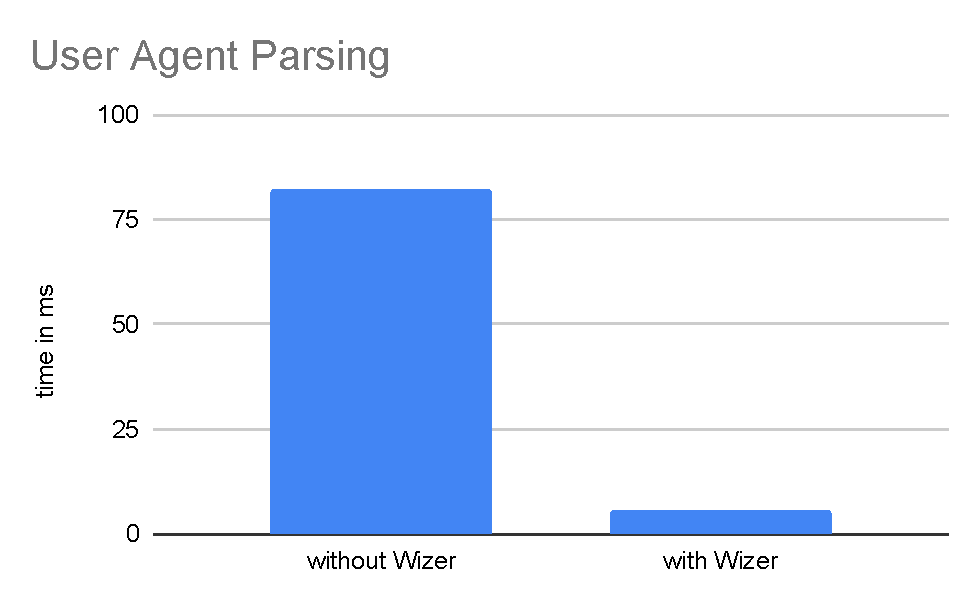
\includegraphics[width=0.6\linewidth]{images/runtimes/UAP.pdf}
	\caption{User Agent Parsing benchmark}
	\label{fig:uap-bench}
\end{figure}


\section{Comparison to V8 Isolates}
\label{sec:v8-comparison}
A V8 isolate is a separate instance of the V8 engine that has its own memory, garbage collector, and global object \cite{a2021_isolate}. An isolate can run scripts in a safe and isolated environment, without interfering with other isolates \cite{cloudflareinc_2023_how}. An isolate also has its own state, which means that objects from one isolate cannot be used in another isolate. When V8 is initialized, a default isolate is created and entered, but you can also create your own isolates using the V8 API \cite{a2021_isolate}.

\begin{figure}[H]
	\centering
		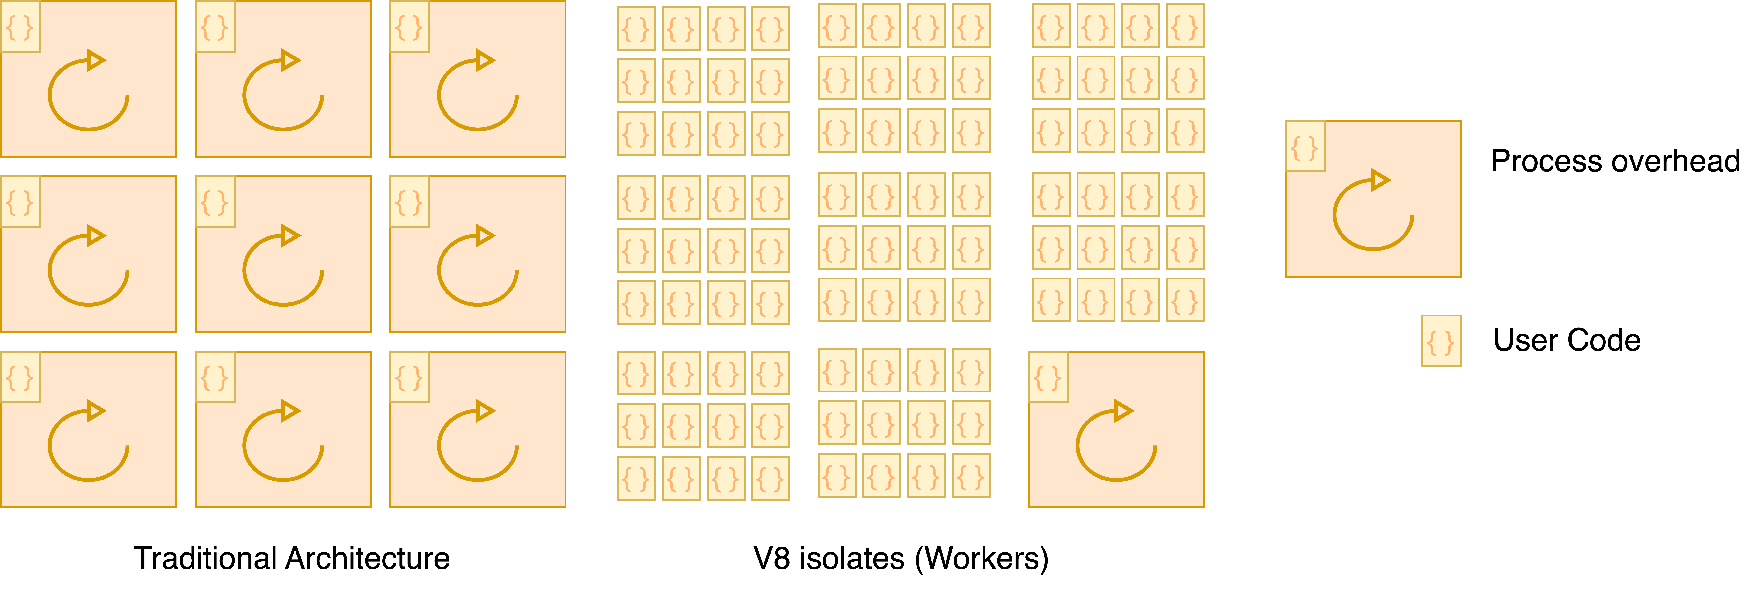
\includegraphics[width=\textwidth,height=\textheight,keepaspectratio]{images/runtimes/v8-isolates.pdf}
	\caption{containerized vs. \gls{V8} \glspl{isolate} figure redrawn from \cite{cloudflareinc_2023_how}}
	\label{fig:v8-isolates}
\end{figure}

\subsection{Advantages and disadvantages}
\label{sec:advantages-disadvantages}
\chapter{WebAssembly Serverless Platform Design}
\label{chap:poc}

In this chapter, the proof of concept for a simple \gls{serverless} compute platform using WebAssembly technology will be explored. For simplicity, the platform runs on an HTTP server to redirect HTTP requests to specific WebAssembly modules. For this, we will use Wasmtime \cite{bytecodealliance_2022_wasmtime} as the WebAssembly runtime, but we could also use Wasmer \cite{wasmerinc_2023_wasmer}. Since Wasmtime does only have Rust integration, we will use the Rust language along with the popular Rust web framework, "Actix-web \cite{actixteam_actix}", due to its lightweight and fast nature. As mentioned in the previous chapter, Wasmtime offers excellent support for the latest WASI standards and features. 

As Figure \ref{fig:poc} illustrates, this proof of concept assumes that there will be a function registry service that stores the ahead-of-time compiled \gls{WebAssembly} binaries. Additionally, a serverless platform needs to be distributed; therefore, API gateways and load balancers are necessary to serve requests across the network. Nonetheless, this proof of concept primarily focuses on the WebAssembly aspect of the platform, leaving the deployment platform, API gateway and load balancers outside the scope of the discussion. 
%
\begin{figure}[htbp]
	\centering
		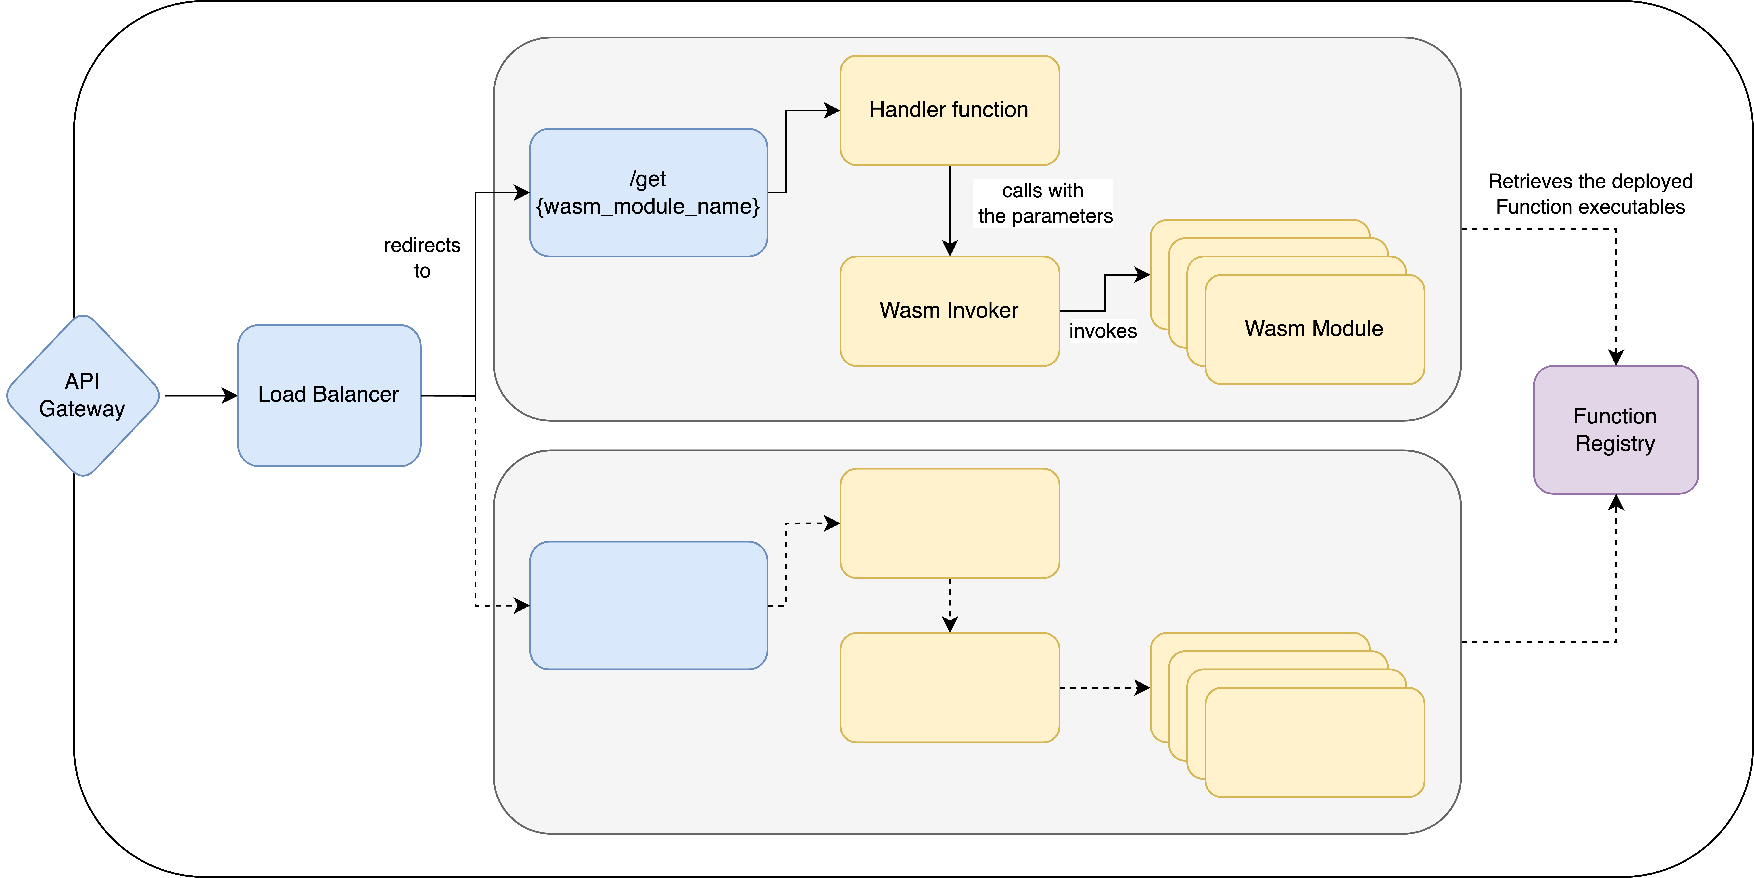
\includegraphics[width=1\linewidth]{images/poc/poc.pdf}
	\caption{Execution flow of the simple POC serverless platform, inspired by \cite[p. 142]{gackstatter_2022_pushing}}
	\label{fig:poc}
\end{figure}
%
The platform has a single endpoint that accepts HTTP requests with a Wasm module name in the path and query parameters. The endpoint will then load the Wasm module from the same directory and call the defined \texttt{invoke\_wasm\_module} in listing \ref{lst:poc-invocation}. This function is the main part of our platform, it is responsible for creating a Wasmtime runtime engine and linker, adding the WASI APIs to the linker. The function then creates a WASI context with the query parameters and loads the module with the file name. The linker is used to link the Wasm module with the later created instance together. There is also a buffer that will be used to store the response from the Wasm module.
%
\begin{lstlisting}[frame=lines, style=Rust, caption={invocation function}, showstringspaces=false, label={lst:poc-invocation}, captionpos=b]
fn invoke_wasm_module(wasm_module_name: String, params: HashMap<String, String>) -> Result<String> {
    let engine = Engine::default();
    let mut linker = Linker::new(&engine);
    wasmtime_wasi::add_to_linker(&mut linker, |s| s)?;

    let stdout_vec_buf: Vec<u8> = vec![]; // a buffer that will contain the response
    let stdout_vec_mutex = Arc::new(RwLock::new(stdout_vec_buf));
    let stdout = WritePipe::from_shared(stdout_vec_mutex.clone());

    // params to array
    let envs: Vec<(String, String)> = params
        .iter()
        .map(|(key, value)| (key.clone(), value.clone()))
        .collect();

    let wasi = WasiCtxBuilder::new()
        .stdout(Box::new(stdout))
        .envs(&envs)?
        .build();
    let mut store = Store::new(&engine, wasi);

    let module = Module::from_file(&engine, &wasm_module_name)?;
    linker.module(&mut store, &wasm_module_name, &module)?;

    run_wasm_module(&mut store, &module, &linker).unwrap();

    // get the response
    let mut buffer: Vec<u8> = Vec::new();
    stdout_vec_mutex
        .read()
        .unwrap()
        .iter()
        .for_each(|i| buffer.push(*i));

    let s = String::from_utf8(buffer)?;
    Ok(s)
}
\end{lstlisting}
%
Directly after, we then call the \texttt{run\_wasm\_module} function shown in \ref{lst:poc-start}. This is where the linker links the module with the newly created instance. The instance is used to search for the start function, the "\_start" function is the starting point of the Wasm modules. It will call the function and return the result. The result is then stored in the buffer and returned to the caller.
%
\begin{lstlisting}[frame=lines, style=Rust, caption={calling the wasm start function}, showstringspaces=false, label={lst:poc-start}, captionpos=b]
fn run_wasm_module(
    mut store: &mut Store<WasiCtx>,
    module: &Module,
    linker: &Linker<WasiCtx>,
) -> Result<()> {
    let instance = linker.instantiate(&mut store, module)?;
    let instance_main = instance.get_typed_func::<(), ()>(&mut store, "_start")?;
    Ok(instance_main.call(&mut store, ())?)
}
\end{lstlisting}
%
To test the platform, we can use any WASI complaint Wasm binary. The following AssemblyScript file contains a simple statement that outputs "Hello World!" on the terminal. The AssemblyScript compiler will compile the file to a WASI complaint Wasm binary. For this we will also need the "wasi-shim" which is a standalone dependency.
%
\begin{lstlisting}[frame=lines, style=JavaScript, caption={AssemblyScript file with a simple console output}, showstringspaces=false, label={lst:as-hello-world}, captionpos=b]
// calling AssemblyScript's console.log, 
// which calls the corresponding WASI interface
console.log('Hello World!');
\end{lstlisting}

\section{Wind-up}

This example shows how easy it is to create a simple \gls{serverless} platform that can invoke any WASI complaint Wasm module. The above Wasm module example was written in AssemblyScript, but in fact, we can use any language that compiles to Wasm and its WASI complaint. If we build this project with the highest compiler optimization, then the resulting binary is only 15 MB in size. This is a modest size for a serverless platform, with less than 80 lines of code. If we run the server and call the mentioned "hello-world" example, we get the following result:
\begin{lstlisting}[frame=lines]
curl -w %{time_total}\\n  http://localhost:8000/hello-world
Hello World!
0.009886
\end{lstlisting}

The result contains the response which, in this case is "Hello World!" and the measured time until the response was received. The measured time is around 10 milliseconds and a deviation of ±15\%. The response time is quite fast, but we should consider the following points:
\begin{itemize}
    \item The server is running on a local machine, with more resources (M1 Pro CPU and 32 GB RAM) than a typical \gls{edge computing} device
    \item The server lacks various features typically associated with a \gls{serverless} platform, therefore it has less overhead than a typical serverless platform
    \item The Wasm module is very simple and does not contain any heavy computation
    \item The large portion of the response time is caused by the Actix Web framework
\end{itemize}

To concrete the last point, we can run the same test without the Wasmtime runtime and the Wasm module. This time we will use the Actix Web framework to return the "Hello World!" string directly and we use the same optimization level as before. The result is shown in the following listing:

\begin{lstlisting}[frame=lines]
curl -w %{time_total}\\n  http://localhost:8000/hello-world
Hello world!
0.005646
\end{lstlisting}

This time the response time is around 6 milliseconds with a deviation of ±10\%. This shows that the Actix Web framework is responsible for 60\% of the response time compared to the previous test setup. This is not surprising, as the Actix Web framework is a full-fledged web framework with many features. 

This is as an excellent starting point for running more precise measurements on the actual runtime in the next chapter, with the aim of gathering a more better picture of the performance of various factors.

\chapter{Evaluation}
\label{chap:evaluation}

In this chapter, we will conduct our evaluation in two parts. In the first part, we will evaluate the performance of different WebAssembly runtimes. In the second part, we will evaluate the performance of the WebAssembly-deployed functions compared to other non-WebAssembly functions.

\section{Goals}
\label{sec:goals}
%
Referring back to our research objectives from \autoref{sec:research-objectives}, the goals of this evaluation are to answer the following questions derived from the research question:
\begin{enumerate}
    \item What is the startup time of a simple \gls{WebAssembly} module?
    \item How do different programming languages compare?
    \item How do various runtimes compare to each other?
    \item How do the WebAssembly runtimes compare to native code?
    \item How does a WebAssembly-powered cloud platform measure up against a V8-powered cloud platform and a cloud platform with microVMs?
\end{enumerate}

\section{Methodology}
\label{sec:methodology}

To answer the above questions, we need to perform a series of different benchmarks. Each benchmark is targeted at answering a specific question. In \autoref{chap:runtimes}, we described the different runtimes with the corresponding compilation models, that we will be using in this evaluation. The next subsections will elaborate on the distinction between microbenchmarks and macrobenchmarks, as well as their application in answering the questions in \autoref{sec:goals}.

\begin{itemize}
    \item \textbf{Microbenchmarks}: Microbenchmarking is a technique used to measure the performance of a small function or a unit of code. It has the advantage of precisely measuring the performance of a specific function or code snippet. However, it can be difficult to extrapolate the results to a real-world scenario. Results from a specific scenario can look very different from the overall performance of a system. The evaluation does contain some microbenchmarks, but the main focus is on macrobenchmarks.
    \item \textbf{Macrobenchmarks}: Macrobenchmarking is not a well-defined term. It can be defined as a type of benchmark that measures the performance of a whole critical path. It is a more realistic approach to compare different systems with similar setups. The drawback of macrobenchmarks is that the results include the performance of the entire system, which is influenced by a lot of variables. To interpret the results, we will first try to subtract the noise and the system's overhead, and then we will compare the results with those of the microbenchmarks.
\end{itemize}

\section{Setup}
\label{sec:setup}

The evaluation setup consists of an AWS EC2 t2.medium instance, deployed on eu-central1 which is located in Frankfurt Germany. The instance is running Ubuntu 22.04 LTS with 2 vCPU and 4 GB of RAM. This instance is used to send requests and conduct benchmarks on different cloud platforms. The advantage of using a ec2 instance is the location. The latency between the ec2 instance and the cloud platforms is very low as shown in \autoref{fig:eval:setup}. The \gls{ICMP} packets have an average round-trip time of 1ms for Fastly, 1.35ms for Cloudflare, and 0.3ms for AWS, as the functions are served by a node in the same availability zone.

Additionally, we ran the benchmarks on this t2.medium instance to measure the runtime performance because it provides a comparable environment with the minimal required resources, to perform the runtime benchmarks. \autoref{fig:eval:setup} shows the deployment setup:

\begin{figure}[htbp]
    \centering
        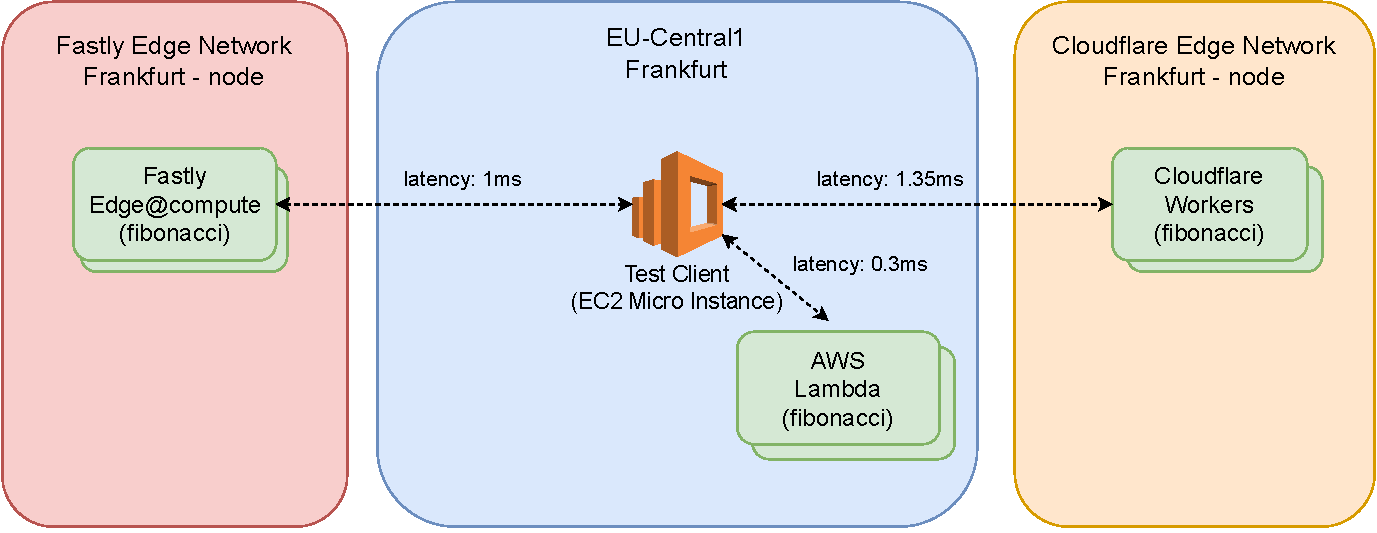
\includegraphics[width=1\linewidth]{images/evaluation/evaluation_setup.drawio.pdf}
    \caption{Deployment setup of the serverless functions}
    \label{fig:eval:setup}
\end{figure}

Moreover, we used a MacBook Pro with M1 Pro CPU and 32GB of RAM to run the runtime benchmarks locally. The benchmarks were executed while the MacBook was plugged into the power supply, and no other major processes were running during the benchmarking process. The M1 Pro CPU is an ARM-based CPU, which is different from the t2.medium's Intel x86 CPU. The results of the two setups cannot be compared directly, but we can use them as a high-level comparison to inspect factors like CPU architecture compatibility and identify any significant outliers. We have tried to perform the benchmarks on a Raspberry PI 2, but the ARM 32-bit architecture is not supported by runtimes like Wasmtime and Wasmer. Aside from that, we also tried a more limited setup with t2.micro instance, but the benchmark code did not compile in a reasonable time. The t2.medium instance is the smallest instance that can run the benchmarks in a reasonable time. 

\section{Criterion}
\label{sec:criterion}

Criterion.rs \cite{heisler_2023_criterionrs} is a statistics-driven benchmarking library for Rust. In our evaluation, Criterion is used to measure the performance of different runtimes. Criterion is a powerful tool that can be employed to measure the performance of a function or a code snippet. Criterion.rs is inspired by Haskell's criterion library. The library provides HTML reports with statistical analysis of the benchmark results, including the mean, median, standard deviation, as well as the regression with previous runs. Moreover, we utilize the library's utility functions such as \texttt{black\_box} to prevent the compiler from optimizing the code away.

Criterion process consists of four phases:

\begin{itemize}
    \item \textbf{Warmup}: In the warmup time the routine is repeatably executed for a given time. This gives the CPU, OS caches and also the JIT compiler if present, time to adapt and optimize the code.
    \item \textbf{Measurement}: Similar to the warmup time the code is repeatably executed in this phase, but unlike the warmup time, the measurement results will be used for analysis. The measurements consists of many samples. Each sample has one or multiple iteration of routines. 
    \item \textbf{Analysis}: This is the phase where the statistical analysis is performed. Values outside of the 25th and 75th percentile are classified as outliers. Values outside of the 5th and 95th percentile are classified as severe outliers. The mean, median, standard deviation, and the regression metrics with previous runs are calculated in this phase.
    \item \textbf{Comparison}: In this phase the statistics of the current run are compared to the previous runs. The comparison is performed using a regression analysis. The results of the comparison are shown in the HTML report and in console output.
\end{itemize}

\section{Benchmarks}
\label{sec:benchmarks}

In this section, we will perform the benchmarks that address the questions outlined in \autoref{sec:goals}. The benchmarks are split into two categories: \textit{runtime} and \textit{serverless platform}. Under the \textit{runtime} category, we will measure the "cold start" time and conduct performance tests with various workloads. In the \textit{serverless platform} category, we will benchmark the response time and compare the performance of different platforms.

\subsection{Cold Start - Instantiation}
\label{subsec:cold-start}

One of the challenges of this thesis has been to precisely define what "cold start" means and how to measure it. In the context of WebAssembly, we define "cold start" as the time it takes from creating a runtime context to loading the module and executing the module's "start" function. This definition is specifically applicable to WebAssembly and V8 setups. The reason for this specificity is the difference between the WebAssembly runtime and a virtualized solution like Firecracker's microVM, which powers the Lambda and AWS Fargate instances. In a virtualized solution, the "cold start" time is the time it takes to boot the virtual machine and load the application. In the case of WebAssembly, the runtime is already running, and the module is loaded into the runtime.

As mentioned before, we utilized the criterion library to measure the instantiation process. Initially, we created a \textit{WAT} file (as shown in \autoref{lst:eval-small-memory}) that included a small memory and a "start" function. The benchmark was executed both locally and on a t2.medium instance. The results are illustrated in \autoref{fig:bench:instantiation:empty-wasm}.

\begin{lstlisting}[frame=lines, style=Wasm, caption={WASI module with small memory}, showstringspaces=false, captionpos=b, label={lst:eval-small-memory}]
    (module
        (memory 1)
        (func (export "_start"))
    )
\end{lstlisting}

\begin{figure}[htbp]
    \centering
        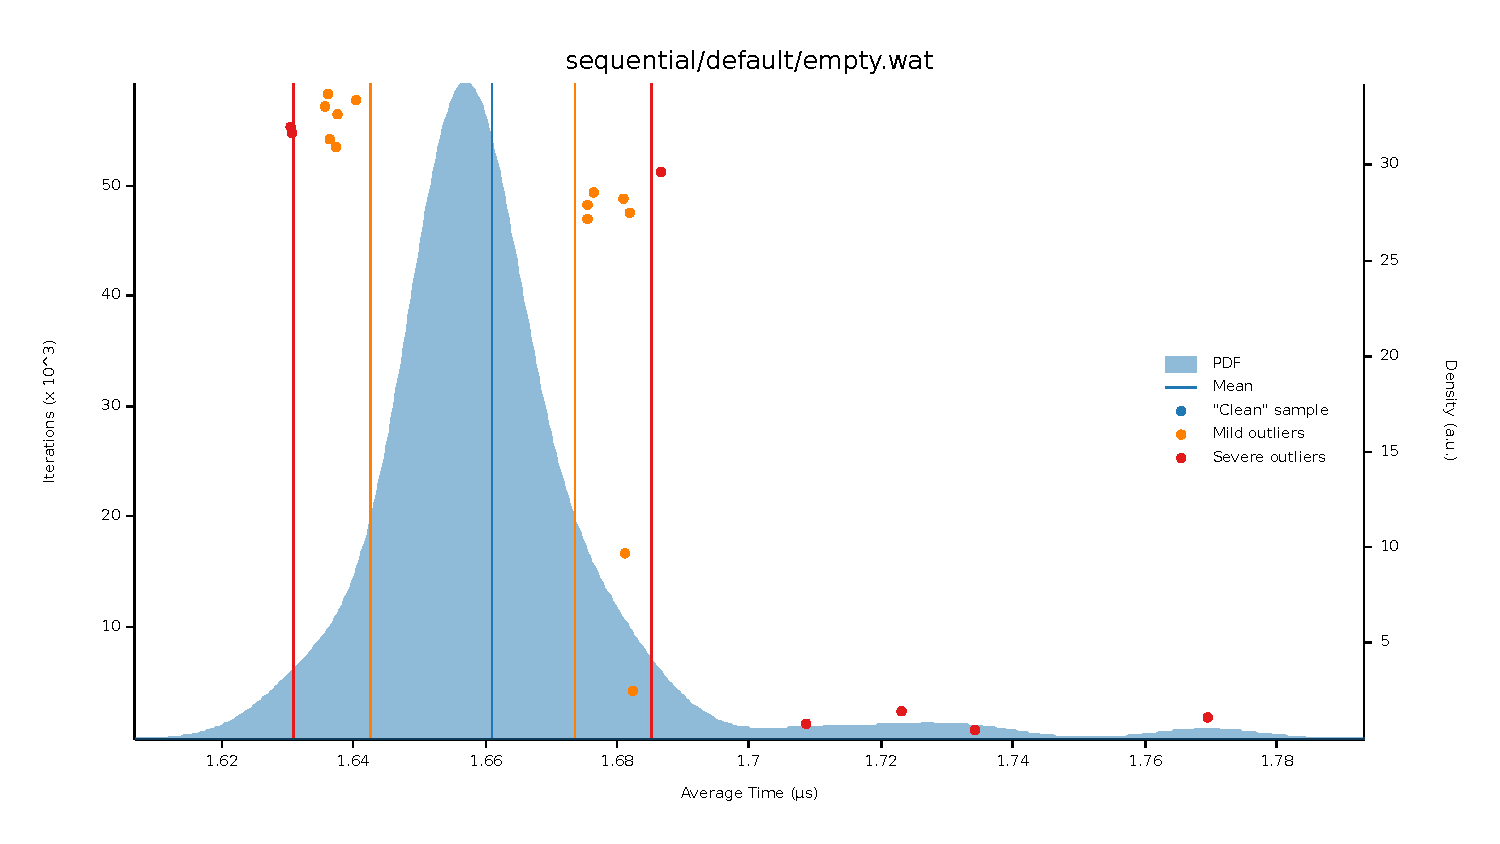
\includegraphics[width=1\linewidth]{images/benches/sequential_default_empty_wasm.pdf}
    \caption{Instantiation distribution of an empty Wasm module with Wasmtime and M1 Pro CPU}
    \label{fig:bench:instantiation:empty-wasm}
\end{figure}

Furthermore, we also conducted an instantiation benchmark, where we first compiled a simple Rust "Hello World" program to a WASI module and then instantiated it using Wasmtime. The results of this benchmark are shown in \autoref{fig:bench:instantiation:wasi}. Please note that we did not measure the compilation time.

Additionally, we performed another benchmark where we defined a \textit{WAT} file with a large data segment and memory. The results for this benchmark are included in the appendix section.

\begin{figure}[htbp]
    \centering
        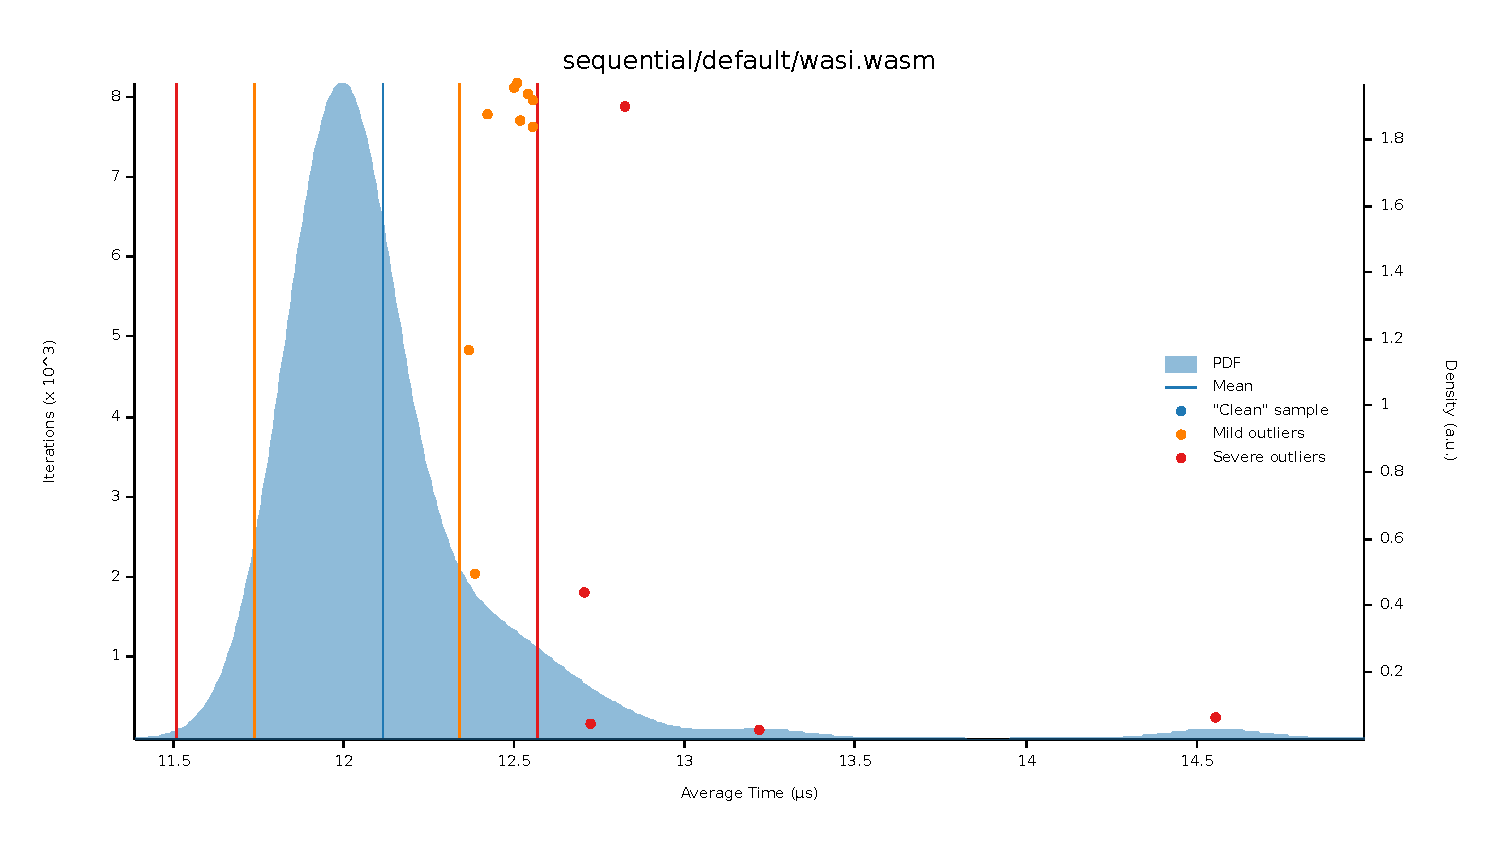
\includegraphics[width=1\linewidth]{images/benches/sequential_default_wasi.pdf}
    \caption{Instantiation distribution of a WASI module with Wasmtime and M1 Pro CPU}
    \label{fig:bench:instantiation:wasi}
\end{figure}


\subsection{Execution Performance}
\label{subsec:executation-performance}

In this section, we will assess the execution performance of different runtimes. Once again, we will use the criterion library for analysis. For this evaluation, we have created both an executable binary and an executable Wasm module. Both the native binary and the Wasm module contain the benchmark function. To ensure realistic production performance, we compiled with the \texttt{--release} flag. Moreover, the Wasm module was automatically optimized using \texttt{wasm-opt}. During benchmarking, the criterion's \texttt{black\_box} utility is used to prevent the compiler from optimizing the code away.

For this evaluation, we have chosen the following runtimes: Wasmtime and Wasmer as the JIT runtimes, Wasm3 as the interpreter runtime, and WasmEdge as the AOT runtime. The benchmarks were conducted using the following functions:

\subsubsection{Fibonacci}

The Fibonacci function is a well-known benchmark used to assess the performance of a runtime. It is chosen for two main reasons: Firstly, it involves a recursive computation, making it a CPU-intensive task. Secondly, it is a simple function that can be easily understood and implemented in any environment.

\subsubsection{Blake3}

Blake3 is an efficient and fast cryptographic hash function. With the increasing use of cryptographic functions in modern applications, it becomes important to measure the performance of such functions. As a deterministic one-way function, Blake3 hashes a "Hello World" string in the benchmark. Unlike the Fibonacci function, Blake3 is expected to execute much faster, leading us to assume that an interpreter runtime or an AOT runtime may have an advantage over a JIT runtime. 

The results of this evaluations are shown in \autoref{fig:eval:t2medium-fib_40}, \autoref{tab:t2-medium-fibonacci} and \autoref{tab:blake3}. We will discuss the results in \autoref{sec:discussion}.

\begin{figure}[htbp]
    \centering
        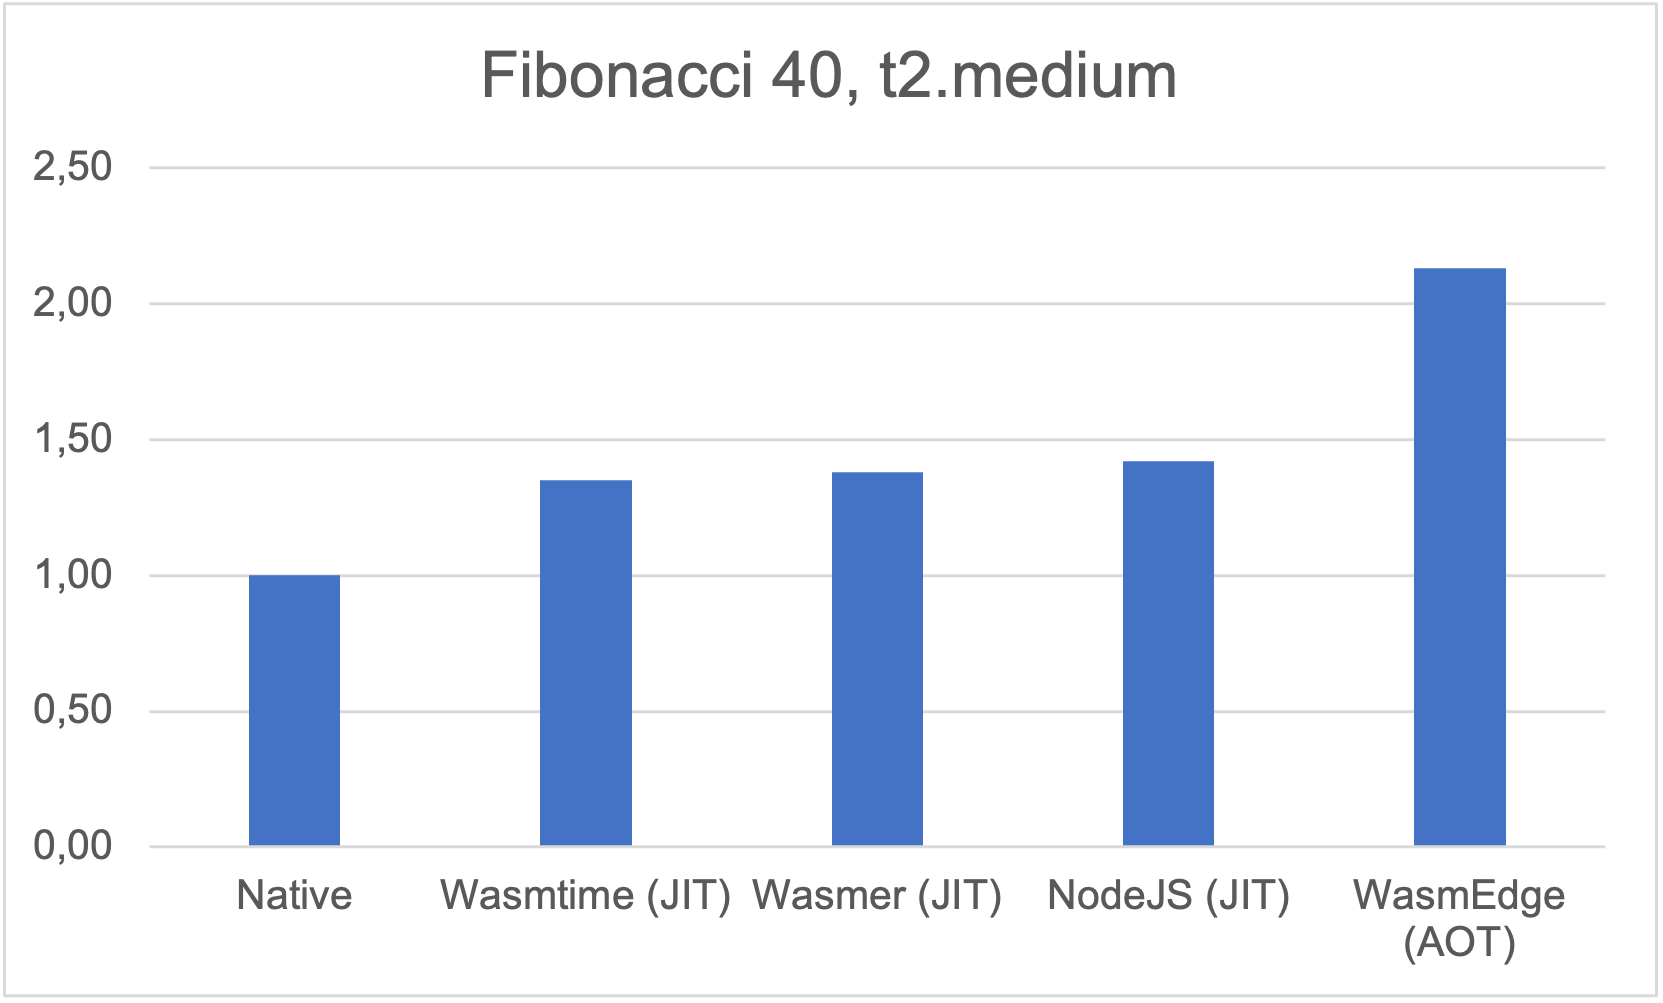
\includegraphics[width=1\linewidth]{images/benches/t2medium_fib_40.png}
    \caption{Runtime comparison on t2.medium: Fibonacci 40 results, excluding Wasm3}
    \label{fig:eval:t2medium-fib_40}
\end{figure}

\begin{table}[]
    \begin{tabular}{|lll|l|lll|}
    \cline{1-3} \cline{5-7}
    \multicolumn{3}{|c|}{\textbf{Fibonnaci 40, t2.medium}}                                           & \multirow{8}{*}{} & \multicolumn{3}{c|}{\textbf{Fibonnaci 32, t2.medium}}                                           \\ \cline{1-3} \cline{5-7} 
    \multicolumn{1}{|l|}{\textbf{Runtime}}  & \multicolumn{1}{l|}{\textbf{Baseline}} & \textbf{Time} &                   & \multicolumn{1}{l|}{\textbf{Runtime}}  & \multicolumn{1}{l|}{\textbf{Baseline}} & \textbf{Time} \\ \cline{1-3} \cline{5-7} 
    \multicolumn{1}{|l|}{\textbf{Native}}   & \multicolumn{1}{l|}{1.00}              & 396.1±0.42ms  &                   & \multicolumn{1}{l|}{\textbf{Native}}   & \multicolumn{1}{l|}{1.00}              & 9.11±0.02ms   \\ \cline{1-3} \cline{5-7} 
    \multicolumn{1}{|l|}{\textbf{Wasmtime}} & \multicolumn{1}{l|}{1.35}              & 534.74±2.24ms &                   & \multicolumn{1}{l|}{\textbf{Wasmtime}} & \multicolumn{1}{l|}{1.31}              & 11.92±1.56ms  \\ \cline{1-3} \cline{5-7} 
    \multicolumn{1}{|l|}{\textbf{Wasmer}}   & \multicolumn{1}{l|}{1.38}              & 546.61±2.61ms &                   & \multicolumn{1}{l|}{\textbf{Wasmer}}   & \multicolumn{1}{l|}{1.33}              & 12.1±1.74ms   \\ \cline{1-3} \cline{5-7} 
    \multicolumn{1}{|l|}{\textbf{NodeJS}}   & \multicolumn{1}{l|}{1.42}              & 562.46±2.41ms &                   & \multicolumn{1}{l|}{\textbf{NodeJS}}   & \multicolumn{1}{l|}{1.45}              & 13.2±2.56ms   \\ \cline{1-3} \cline{5-7} 
    \multicolumn{1}{|l|}{\textbf{WasmEdge}} & \multicolumn{1}{l|}{2.13}              & 843.69±4.21ms &                   & \multicolumn{1}{l|}{\textbf{WasmEdge}} & \multicolumn{1}{l|}{2.21}              & 20.11±3.23ms  \\ \cline{1-3} \cline{5-7} 
    \multicolumn{1}{|l|}{\textbf{Wasm3}}    & \multicolumn{1}{l|}{4.82}              & 1909.2±8.52ms &                   & \multicolumn{1}{l|}{\textbf{Wasm3}}    & \multicolumn{1}{l|}{4.51}              & 41.04±2.51ms  \\ \cline{1-3} \cline{5-7} 
    \end{tabular}
    \caption{Runtime Benchmark: Fibonacci 40 and 32 on t2.medium; Wasmtime, Wasmer, NodeJS (JIT), WasmEdge (AOT), Wasm3 (Interpreter)}
    \label{tab:t2-medium-fibonacci}
\end{table}


\begin{table}[]
    \begin{tabular}{|lll|l|lll|}
    \cline{1-3} \cline{5-7}
    \multicolumn{3}{|c|}{\textbf{Blake3, M1 PRO CPU}}                                                & \multirow{8}{*}{} & \multicolumn{3}{c|}{\textbf{Blake3, t2.medium}}                                                  \\ \cline{1-3} \cline{5-7} 
    \multicolumn{1}{|l|}{\textbf{Runtime}}  & \multicolumn{1}{l|}{\textbf{Baseline}} & \textbf{Time} &                   & \multicolumn{1}{l|}{\textbf{Runtime}}  & \multicolumn{1}{l|}{\textbf{Baseline}} & \textbf{Time}  \\ \cline{1-3} \cline{5-7} 
    \multicolumn{1}{|l|}{\textbf{Native}}   & \multicolumn{1}{l|}{1.00}              & 83.8±1.86ns   &                   & \multicolumn{1}{l|}{\textbf{Native}}   & \multicolumn{1}{l|}{1.00}              & 114.7±0.19ns   \\ \cline{1-3} \cline{5-7} 
    \multicolumn{1}{|l|}{\textbf{NodeJS}}   & \multicolumn{1}{l|}{1.10}              & 92.3±2.24ns   &                   & \multicolumn{1}{l|}{\textbf{NodeJS}}   & \multicolumn{1}{l|}{1.32}              & 150.084±1.56ns \\ \cline{1-3} \cline{5-7} 
    \multicolumn{1}{|l|}{\textbf{Wasmtime}} & \multicolumn{1}{l|}{1.13}              & 94.3±2.61ns   &                   & \multicolumn{1}{l|}{\textbf{Wasmtime}} & \multicolumn{1}{l|}{1.41}              & 161.727±1.74ns \\ \cline{1-3} \cline{5-7} 
    \multicolumn{1}{|l|}{\textbf{Wasmer}}   & \multicolumn{1}{l|}{1.35}              & 113.13±2.41ns &                   & \multicolumn{1}{l|}{\textbf{Wasmer}}   & \multicolumn{1}{l|}{1.46}              & 167.462±2.56ns \\ \cline{1-3} \cline{5-7} 
    \multicolumn{1}{|l|}{\textbf{WasmEdge}} & \multicolumn{1}{l|}{2.05}              & 171.5±4.21ns  &                   & \multicolumn{1}{l|}{\textbf{WasmEdge}} & \multicolumn{1}{l|}{2.15}              & 246.605±3.23ns \\ \cline{1-3} \cline{5-7} 
    \multicolumn{1}{|l|}{\textbf{Wasm3}}    & \multicolumn{1}{l|}{4.82}              & 403.91±8.52ns &                   & \multicolumn{1}{l|}{\textbf{Wasm3}}    & \multicolumn{1}{l|}{4.97}              & 570.059±2.51ns \\ \cline{1-3} \cline{5-7} 
    \end{tabular}
    \caption{Runtime Benchmark: Blake3 on M1 PRO and t2.medium; Wasmtime, Wasmer, NodeJS (JIT), WasmEdge (AOT), Wasm3 (Interpreter)}
    \label{tab:blake3}
\end{table}

\subsection{Evaluating Serverless Platforms}
\label{subsec:evaluating-serverless-platforms}

Evaluating various serverless platforms is a challenging task, because there are a handful of variable factors that can influence the measurements.

We deployed the same functions on different platforms and with different programming languages. The functions were invoked by a timestamp in order to prevent caching of the response by the CDN. The functions were invoked sequentially with a delay of 15 minutes between each invocation. The delay was chosen to prevent warm starts, we conducted a few tests to find the idle time before the functions are terminated. A bash script was used to invoke the functions with curl and write the response metrics into a file. As mentioned in the \autoref{sec:setup} the test instance has a latency of 0.3 to 1.3 milliseconds to the functions. Here is a list of the deployed functions:

\begin{itemize}
    \item \textbf{Fibonacci}: The Fibonacci function calculates the Fibonacci for a given number \textit{n}. The function is implemented in Rust, JavaScript and Go. We deployed the function on Fastly Compute@Edge, Cloudflare Workers (only JavaScript) and AWS Lambda (only JavaScript).
    \item \textbf{Blake3}: The Blake3 function calculates the hash of a given string. We used the string "Hello World". The function is implemented in Rust, JavaScript and Go. We deployed the function on Fastly Compute@Edge, Cloudflare Workers (only JavaScript) and AWS Lambda (only JavaScript).
\end{itemize}

\subsubsection{Curl Performance Metrics}

The curl command is a powerful built-in tool in the bash shell. We use it to send the requests from the test client to each serverless function. An overview of how a request is sent and what processes are involved is shown in \autoref{fig:eval:curl-metrics}. The curl command is executed with the following parameters:
\texttt{curl -w "@curl-format.txt" -o /dev/null -s "https://serverless-function-address.app/"}

the \texttt{curl-format.txt} formats the response. The following metrics are recorded (more details on \cite{speedtestdemon_2021_cheat}):

\begin{itemize}
    \item \textbf{time\_namelookup}: The time in seconds it took from the start until domain resolving was completed.
    \item \textbf{time\_connect}: The time in seconds it took from the start until the three way handshake was completed from the clients perspective.
    \item \textbf{time\_appconnect}: Is the time where the TLS setup is done. The client is able to send the HTTP GET request.
    \item \textbf{time\_starttransfer}: The time it took until the first byte of the response was by curl. This is also known as the TTFB (Time to first byte). If we calculate \texttt{TTFB - (time\_connect - time\_namelookup)} then we get the time it took for the server to process the request.
    \item \textbf{time\_total}: The total time in seconds is the duration between the time the request was sent and the time the last byte of the response was received.
\end{itemize}

These metrics provide valuable insights into the actual performance of the serverless functions and analyze the outliers caused by the network.


\begin{figure}[htbp]
    \centering
        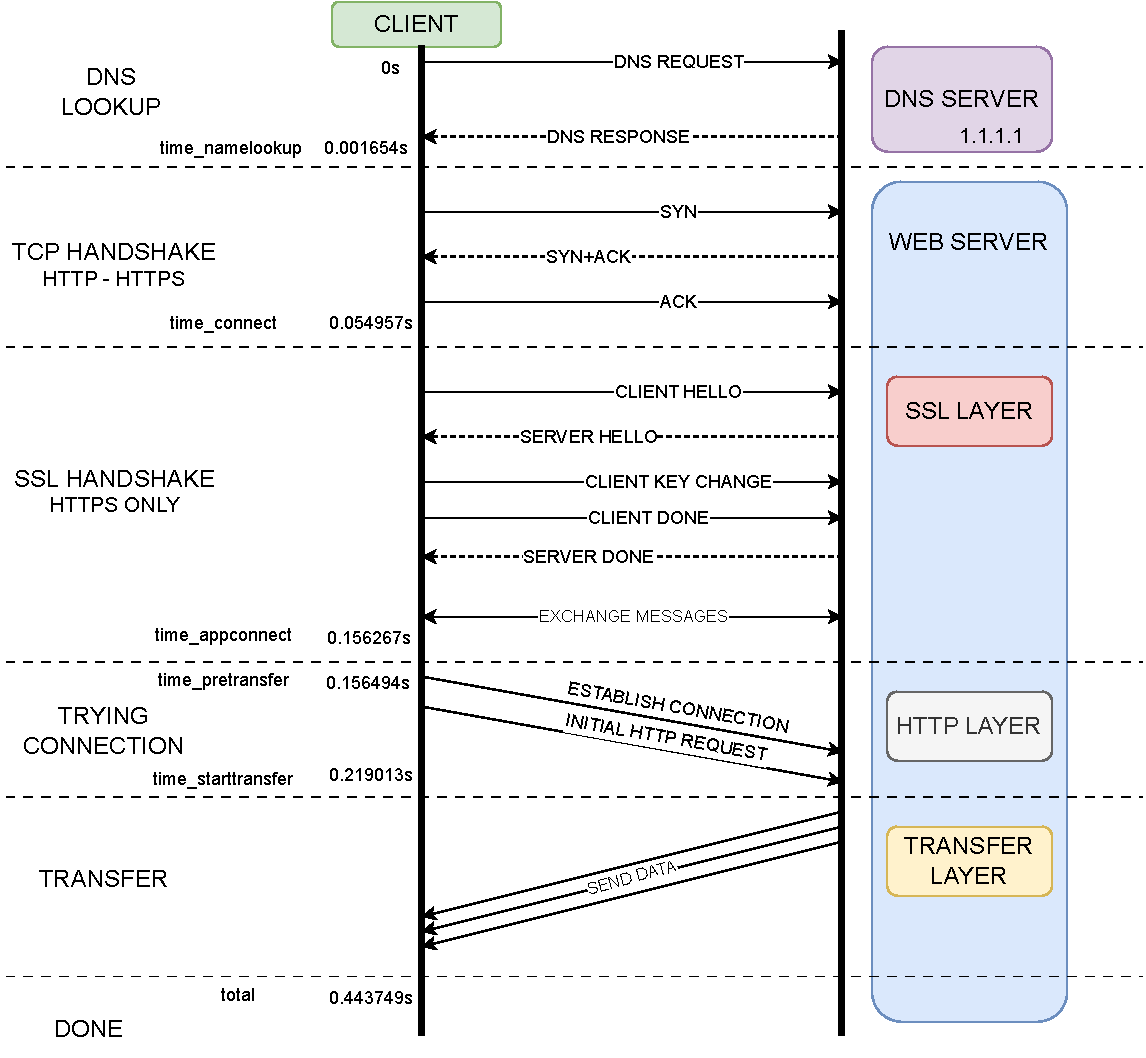
\includegraphics[width=1\linewidth]{images/evaluation/curl_performance_metrics.drawio.pdf}
    \caption{Curl performance metrics visualization, redrawn from \cite{speedtestdemon_2021_cheat}}
    \label{fig:eval:curl-metrics}
\end{figure}

\begin{figure}[htbp]
    \centering
        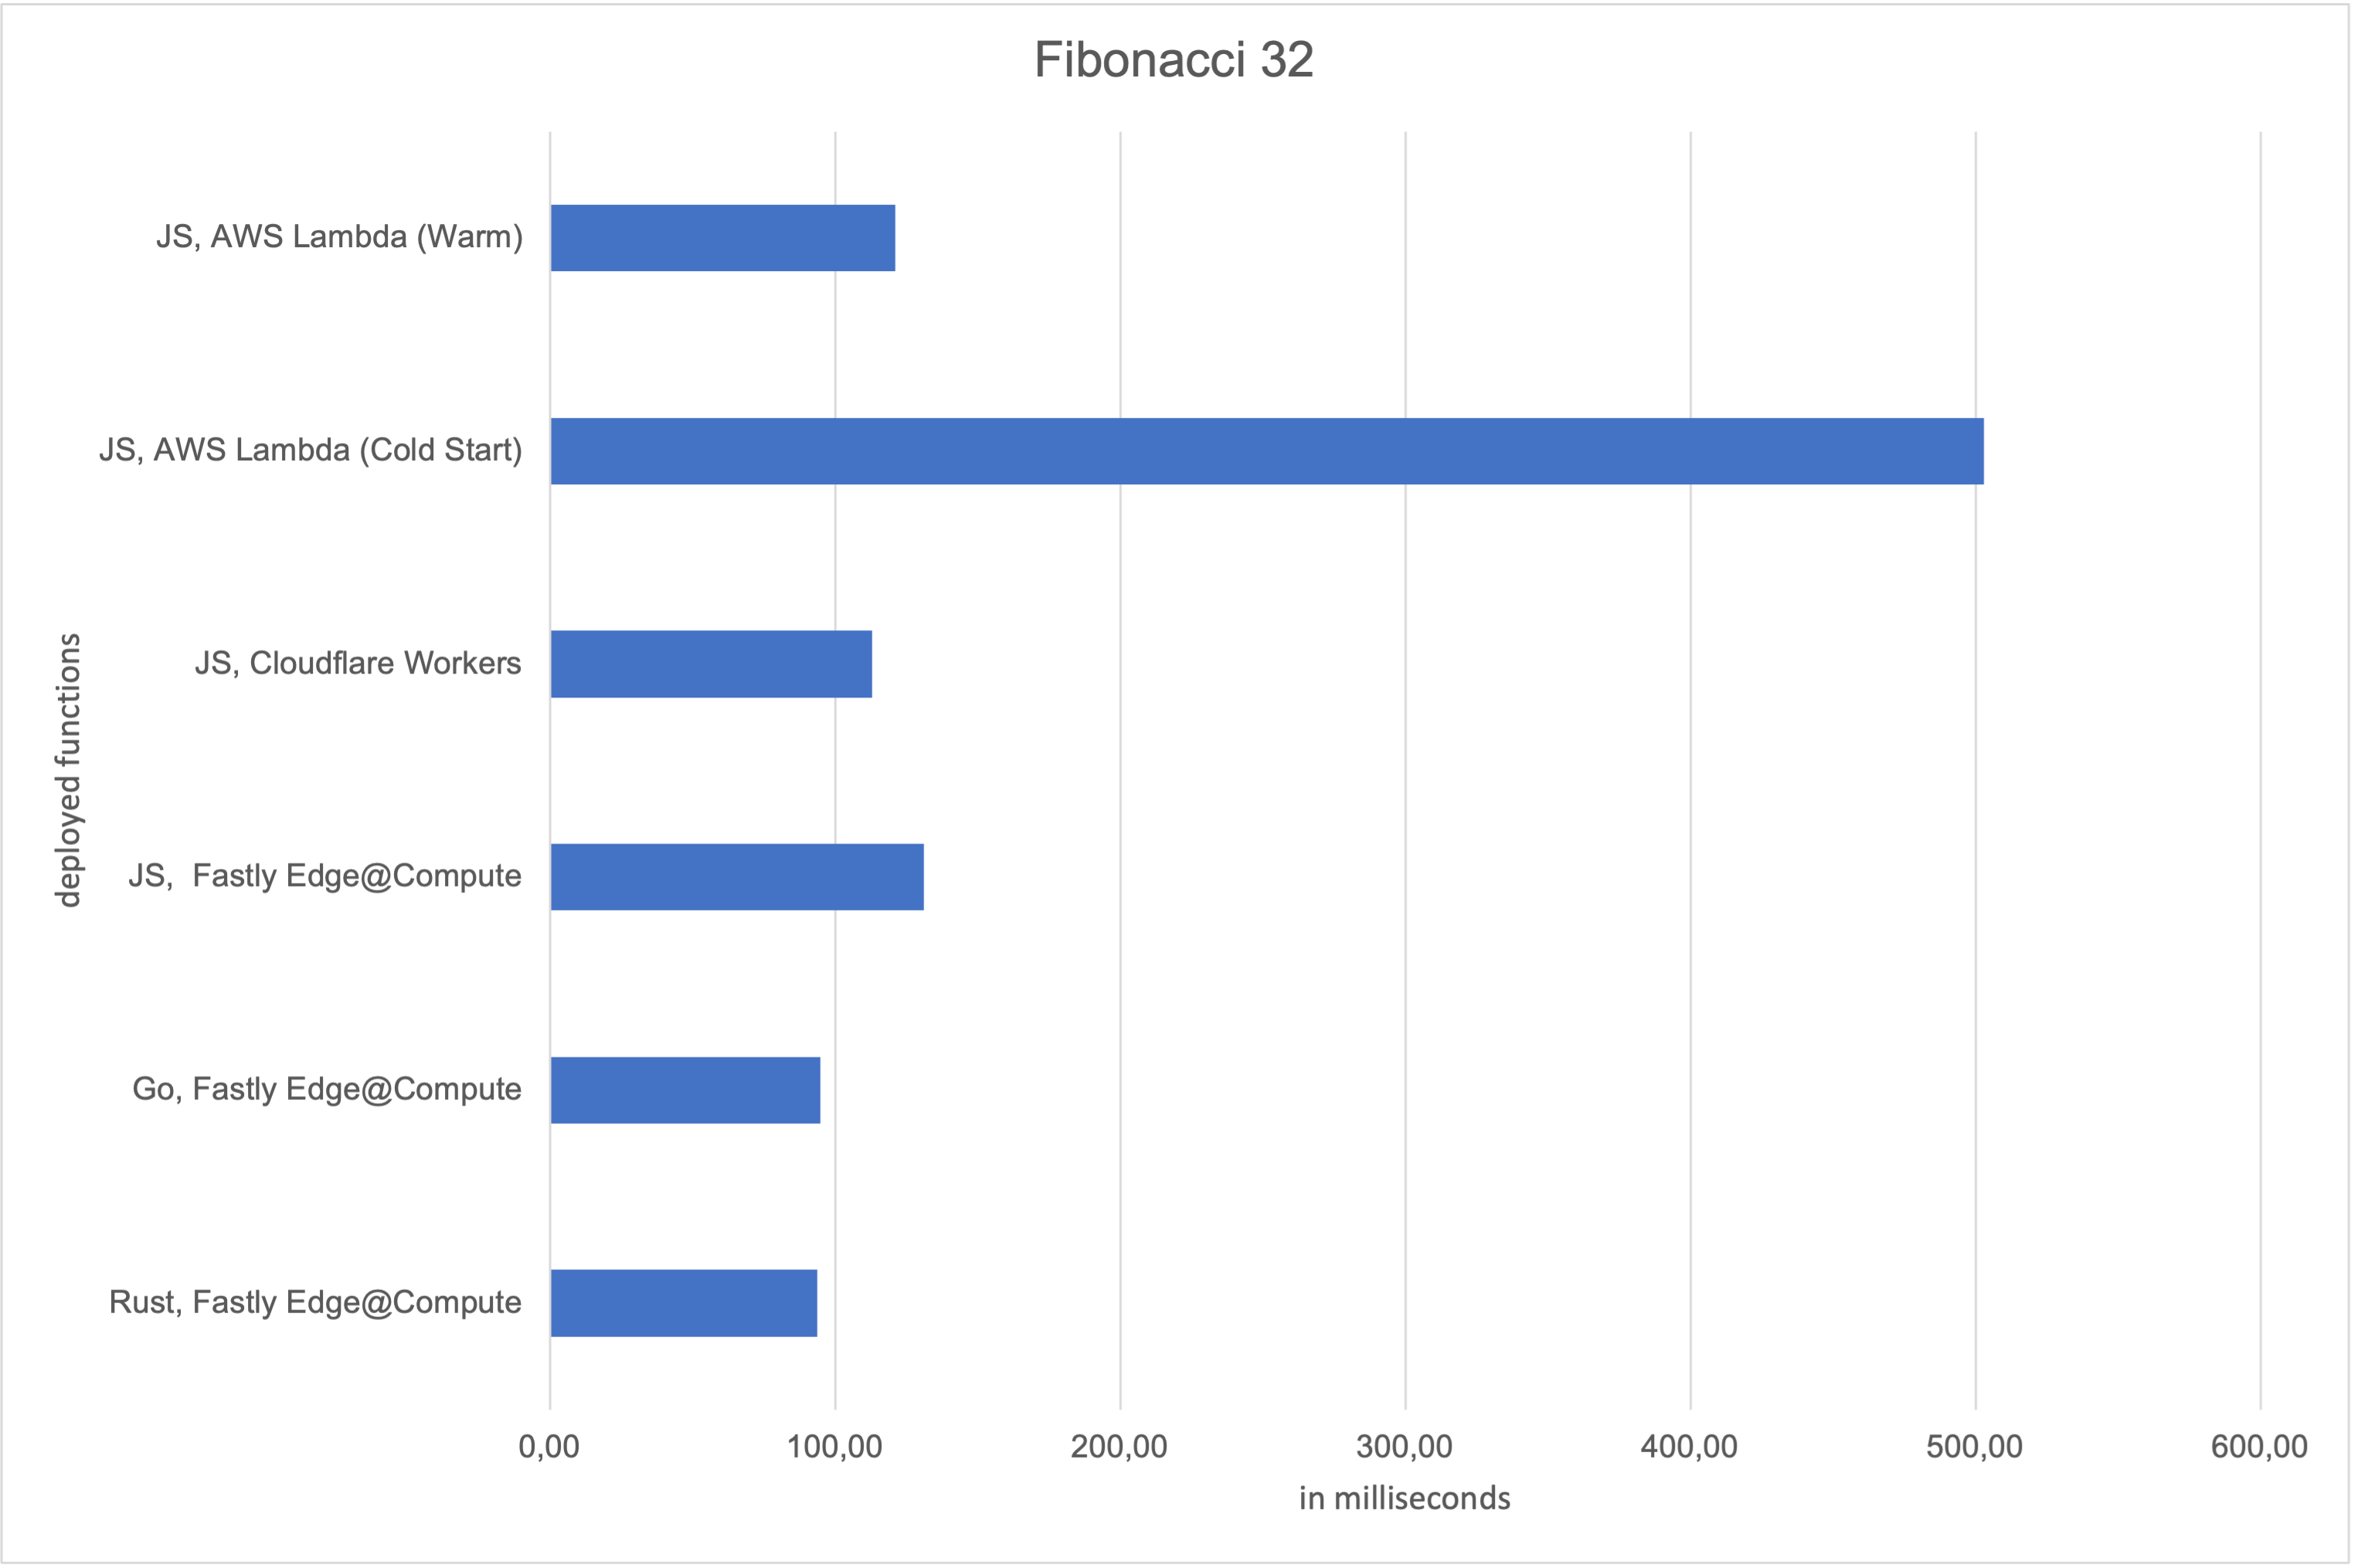
\includegraphics[width=0.95\linewidth]{images/benches/deployed_functions_fib32.png}
    \caption{Derived results of deployed functions: Fibonacci 32, the result is calculated with TTFB - (time connect - time namelookup)}
    \label{fig:eval:deployed-functions}
\end{figure}

\section{Discussion}
\label{sec:discussion}

In this section we will answer the questions from \autoref{sec:goals} and discuss the findings of the evaluation. We will also address the limitations encountered during the evaluation.

\subsection{Evaluation Questions}

\textbf{1. What is the startup time of a simple \gls{WebAssembly} module?}

We evaluated the startup time of a simple \textit{WAT} file, loading a Rust to \gls{wasi}-compiled file, and a Wasm module with a large data segment. These benchmarks, as shown in \autoref{fig:bench:instantiation:wasi}, indicate a startup time ranging from 5 to 40 microseconds overall. Additionally, we evaluated the startup time of deserializing and loading a deserialized Wasm module. The startup time of a deserialized Wasm module is about 98 microseconds for a t2.medium instance (shown in \autoref{fig:bench:instantiation:t2-deserialize-wasi-wasm} in the appendix). Under adverse conditions, we could see a startup time of 1 to 5 milliseconds depending on the size of the Wasm module. The size of a bundled serverless function is typically small, and some cloud providers impose size limits.

\textbf{2. How do different programming languages compare?}

We evaluated the performance of the programming languages Rust, JavaScript, and Go. The performance of these programming languages is similar, with Rust being slightly faster than Go and JavaScript, as shown in \autoref{fig:eval:deployed-functions}.

\textbf{3. How do various runtimes compare to each other?}

The results show that Wasmtime and Wasmer are similar in performance, with Wasmtime being slightly faster than Wasmer. In contrast, Wasm3, as shown in \autoref{tab:blake3}, is the slowest runtime in our evaluation. It is not surprising that Wasm3 is slower than Wasmtime and Wasmer, as Wasm3 is an interpreter runtime with a main focus on small footprint and portability. Wasm3 can find its use case in embedded systems, where the host devices may not be powerful enough to run a JIT compiler. It should be noted that our results show a worse performance for Wasm3 than the results presented in the official GitHub repository \cite{shymanskyy_2023_wasm3}. 

\textbf{4. How do the WebAssembly runtimes compare to native code?}

Initially, we assumed that WebAssembly runtimes are about 30\% slower than native code. However, the results show that WebAssembly runtimes are approximately 40\% slower on long-running tasks and about 35\% slower on short-running tasks, as shown in \autoref{tab:t2-medium-fibonacci}. It is essential to note that WebAssembly runtimes outside of the browser are still in an early stage, and we can expect performance improvements in the future.

Secondly, we did not compile our Wasm module to a native binary, and it is reasonable to anticipate a performance improvement when doing so. This technique is used by the Fastly Compute@Edge platform once the optimized binary is deployed.

\textbf{5. How does a WebAssembly-powered cloud platform measure up against a V8-powered cloud platform and a cloud platform with microVMs?}

Cloudflare's Workers run on V8 isolates, and the only supported language for an isolate is JavaScript. The results show that Cloudflare Workers are slightly faster than the JavaScript version of Fastly Compute@Edge. We believe that the JavaScript runtime of Fastly Compute@Edge is not as mature as the V8 isolates employed by Cloudflare. However, the Rust version of Fastly outperforms the Cloudflare version.

Finally, we compared the performance of Fastly Compute@Edge with AWS Lambda. The results show that the cold start delay of AWS is about 400 milliseconds, as the first request took about 500 milliseconds, and the subsequent request took about 114 milliseconds. Even in a warm state, AWS Lambda is approximately as fast as the Fastly Compute@Edge JavaScript version. The results are shown in \autoref{fig:eval:deployed-functions}.

\subsection{Technical Limitations}

The evaluation was limited to only three languages. We could not use Java for the evaluation because the WasmGC proposal is not merged in the specification.

Furthermore, a criterion dependency did not support the \gls{wasi} target; therefore, we could not use it for plotting the runtime performance evaluation. Instead, we used the stored data to plot the results.
\chapter{Platform Limitations}
\label{chap:limitations}

The component model
\chapter{Vendor lock-in}
\label{chap:vendor-lock-in}

Cloud computing's vendor lock-in issue arises when customers become reliant (i.e., locked-in) on a specific cloud provider's technology implementation. This makes it challenging and costly to switch to another vendor due to legal constraints, technical incompatibilities, or significant expenses in the future. The issue of vendor lock-in in cloud computing has been identified as a major challenge because transferring applications and data to other providers is often an expensive and time-consuming process, making portability and interoperability essential considerations \cite{guest_2013_oracle}.

There are two primary factors contributing to the difficulty of achieving interoperability, portability, compliance, trust, and security in cloud computing. The first is the absence of universally adopted standards, APIs, or interfaces that can leverage the ever-changing range of cloud services. The second is the lack of standardized practices for deployment, maintenance, and configuration \cite{oparamartins_2014_critical}, which creates challenges for ensuring consistency and compatibility across cloud environments. 

\section{Key Motivations for shifting to a new Cloud Provider}
There are various reasons why a customer may contemplate changing their service provider:

\begin{enumerate}
    \item Inconsistent or unreliable service quality
    \item Escalating costs associated with function execution, prompting a search for a more cost-effective alternative.
    \item Runtime issues or limitations encountered with the current provider.
    \item The need to integrate a function with a new back-end service that is only offered by a different provider.
    \item Strategic or support considerations within the organization that may necessitate a switch to a different Cloud provider.
\end{enumerate}

\subsection{Service interoperability}


\subsection{Which parts need to be considered when migrating to a different provider?}
To evaluate the feasibility of switching \Gls{FaaS} providers, it is necessary to examine the modifications needed for the function codebase as well as the adjustments required for the execution configuration, deployment, and triggers.

\subsubsection{Differences in handler function}
Each cloud computing service provider has its own unique function signature that must be adhered to for the code to be executed on their respective cloud platforms. These signatures can vary slightly between different providers. The subsequent Javascript code examples illustrate how input can be read from the event and responses can be sent back for each cloud provider. These examples assume that the function is triggered through an HTTP POST request and with a JSON body conaining "myName" property. \\
The first example is an AWS Lambda Function, the body is within the event object, the function resolves the request by returning an object that contains a "statusCode" property along with a body.

\begin{lstlisting}[frame=lines, style=ES6, caption={Basic AWS Lambda Function}, showstringspaces=false, captionpos=b,]
export const handler = async(event, context) => {
  const input = JSON.parse(event.body);
  return {
      statusCode: 200,
      body: JSON.stringify({
          message: `Hello ${input.myName}`,
      })
  };
};
\end{lstlisting}
The next \gls{serverless} function is running on Google Cloud, the difference is not only in the function signature, but also the fact that the function imports the framework.

\begin{lstlisting}[frame=lines, style=ES6, caption={Basic Gen. 2 Google Cloud Functions}, showstringspaces=false, captionpos=b,]
const functions = require("@google-cloud/functions-framework");

functions.http("/", (req, res) => {
  res.status(200).send({
       message: `Hello ${req.body.myName}`
    });
});
\end{lstlisting}

TODO: short description

\begin{lstlisting}[frame=lines, style=ES6, caption={Basic Cloudflare Workers}, showstringspaces=false, captionpos=b,]
export default {
  async fetch(request, env, ctx) {
      const input = JSON.parse(await request.text());
      return new Response(JSON.stringify({
          message: `Hello, ${input.myName}`,
      }), {
          status: 200,
          headers: {
              "content-type": "application/json",
          },
      });
  },
};
\end{lstlisting}

TODO: short description

\begin{lstlisting}[frame=lines, style=ES6, caption={Basic Fastly Compute@Edge}, showstringspaces=false, captionpos=b,]
addEventListener("fetch", (event) => event.respondWith(handleRequest(event)));

async function handleRequest(event) {
  const request = event.request;
  const input = JSON.parse(await request.text());
  return new Response(JSON.stringify({
    message: `Hello, ${input.myName}`,
  }), { 
    status: 200,
    headers: {
      "content-type": "application/json",
    },
  });
}
\end{lstlisting}

\section{Design principles}
\subsection{Facade pattern}
The \gls{facade} pattern can be used as a mitigation strategy to avoid or reduce \gls{serverless} vendor lock-in. By creating a facade layer between the serverless function and the vendor-specific implementation, it is possible to decouple the function from the vendor's specific implementation details.
The facade layer provides a simplified interface that abstracts the underlying vendor implementation, allowing developers to write code that is agnostic to the specific \gls{serverless} vendor. If the vendor needs to be changed, the facade layer can be modified to adapt to the new vendor-specific implementation without affecting the business logic or the interface of the serverless function. This way, the codebase remains modular, and changing vendors becomes a relatively straightforward task.

\subsection{Adapter pattern}
SvelteKit is a modern web framework that effectively demonstrates the use of the Adapter pattern for deployment. Before deploying a SvelteKit application, it must be adapted to the specific deployment target by selecting an appropriate adapter in the configuration. This allows the application to be bundled with the platform-specific configuration \cite{sveltecommunity_2023_adapter}. 
The code snippet below illustrates the adapter configuration of a SvelteKit application, which enables the framework to be adapted to various cloud providers and allows the community to create new adapters. In this case, the deployment target is a Cloudflare Workers \gls{serverless} function.

\begin{lstlisting}[frame=lines, style=ES6, caption={svelte.config.js SvelteKit adapter configuration}, showstringspaces=false, captionpos=b,]
import adapter from '@sveltejs/adapter-cloudflare-workers';
 
/** @type {import('@sveltejs/kit').Config} */
const config = {
  kit: {
    adapter: adapter({
      // adapter options go here
    })
  }
};
 
export default config;
\end{lstlisting}

\section{The role of Wasm Portability}
\chapter{Related Work}
\label{chap:related-work}


\chapter{Conclusion}
\label{chap:conclusion}


\chapter{Future work}
\label{chap:future-work}

Future work ...

%\clearpage

% --- Bibliography ------------------------------------------------------
\newpage
%IEEE Citation [1]
\bibliographystyle{IEEEtran}
\bibliography{master_thesis}
%for alphanumeric citation eg.: [ABC19]
%\bibliographystyle{alpha}
\addcontentsline{toc}{chapter}{Bibliography}
%\clearpage

% --- Glossary ----------------------------------------------------

%\newpage
\label{chap:glossary}
\printnoidxglossaries
%\printglossary
\addcontentsline{toc}{chapter}{Glossary}
%\clearpage


% --- List of Figures ----------------------------------------------------

\newpage
\listoffigures
\addcontentsline{toc}{chapter}{List of Figures}
%\clearpage


% --- List of Tables -----------------------------------------------------

\newpage
\listoftables
\addcontentsline{toc}{chapter}{List of Tables}
%\clearpage

% --- Appendix A -----------------------------------------------------

\newpage
\backmatter
\appendix
\begin{appendices}
\chapter{Appendix}
\begin{lstlisting}[frame=lines, style=Rust, caption={Simple Proof of Concept Wasm Serverless Platform using Actix and Wasmtime}, showstringspaces=false, captionpos=b,]
use actix_web::{
    get,
    web::{Path, Query},
    App, HttpResponse, HttpServer, Responder,
};
use anyhow::Result;
use std::{
    collections::HashMap,
    io,
    sync::{Arc, RwLock},
};
use wasi_common::{pipe::WritePipe, WasiCtx};
use wasmtime::*;
use wasmtime_wasi::WasiCtxBuilder;

#[actix_web::main]
async fn main() -> io::Result<()> {
    HttpServer::new(|| App::new().service(handler))
        .bind("127.0.0.1:8080")?
        .run()
        .await
}

#[get("/{wasm_module_name}")]
async fn handler(
    wasm_module_name: Path<String>,
    query: Query<HashMap<String, String>>,
) -> impl Responder {
    let wasm_module = format!("{}.wasm", wasm_module_name);
    match invoke_wasm_module(wasm_module, query.into_inner()) {
        Ok(val) => HttpResponse::Ok().body(val),
        Err(e) => HttpResponse::InternalServerError().body(format!("Error: {}", e)),
    }
}

fn run_wasm_module(
    mut store: &mut Store<WasiCtx>,
    module: &Module,
    linker: &Linker<WasiCtx>,
) -> Result<()> {
    let instance = linker.instantiate(&mut store, module)?;
    let instance_main = instance.get_typed_func::<(), ()>(&mut store, "_start")?;
    Ok(instance_main.call(&mut store, ())?)
}

fn invoke_wasm_module(wasm_module_name: String, params: HashMap<String, String>) -> Result<String> {
    // create a wasmtime engine
    let engine = Engine::default();

    let mut linker = Linker::new(&engine);
    wasmtime_wasi::add_to_linker(&mut linker, |s| s)?;

    // create a buffer to store the response
    let stdout_buf: Vec<u8> = vec![];
    let stdout_mutex = Arc::new(RwLock::new(stdout_buf));
    let stdout = WritePipe::from_shared(stdout_mutex.clone());

    // convert params hashmap to an array
    let envs: Vec<(String, String)> = params
        .iter()
        .map(|(key, value)| (key.clone(), value.clone()))
        .collect();

    let wasi = WasiCtxBuilder::new()
        .stdout(Box::new(stdout))
        .envs(&envs)?
        .build();
    let mut store = Store::new(&engine, wasi);

    let module = Module::from_file(&engine, &wasm_module_name)?;
    linker.module(&mut store, &wasm_module_name, &module)?;

    run_wasm_module(&mut store, &module, &linker).unwrap();

    // read the response into a string
    let mut buffer: Vec<u8> = Vec::new();
    stdout_mutex
        .read()
        .unwrap()
        .iter()
        .for_each(|i| buffer.push(*i));
    let s = String::from_utf8(buffer)?;
    Ok(s)
}
\end{lstlisting}


\clearpage
\end{appendices}

\end{document}
